%%%%%%%%%%%%%%%%%%%%%%%%%%%%%%%%%%%%%%%%%
% MEIA Dissertation
% LaTeX Template
% (Jan/2022)
%
% Adapted once again to MEIA/ISEP style (Jan(2022) by:
%  Luiz Faria (lef@isep.ipp.pt)
%
% Adapted to TMDEI/ISEP style (Dec/2015) by
%  Nuno Pereira (nap@isep.ipp.pt) and
%  Paulo Baltarejo (pbs@isep.ipp.pt)
%
% Based on MastersDoctoralThesis Version 1.2 by Vel (vel@latextemplates.com) and
% Johannes Böttcher, downloaded from (21/11/15):
% http://www.LaTeXTemplates.com
%
% This template is originally based on a template by:
% Steve Gunn (http://users.ecs.soton.ac.uk/srg/softwaretools/document/templates/)
% Sunil Patel (http://www.sunilpatel.co.uk/thesis-template/)
%
% Template license:
% CC BY-NC-SA 3.0 (http://creativecommons.org/licenses/by-nc-sa/3.0/)
%
%%%%%%%%%%%%%%%%%%%%%%%%%%%%%%%%%%%%%%%%%
%
%----------------------------------------------------------------------------------------
%	PACKAGES AND OTHER DOCUMENT CONFIGURATIONS
%----------------------------------------------------------------------------------------

\documentclass[
11pt, % The default document font size, options: 10pt, 11pt, 12pt
%oneside, % Two side (alternating margins) for binding by default, uncomment to switch to one side (for drafting/reading purposes)
english, % english for English;
%portuguese,% for Portuguese; delete temporary files if you change language (e.g. 'make clean; make')
singlespacing, % Single line spacing, alternatives: onehalfspacing or doublespacing (for drafting/reading purposes)
%draft, % Uncomment to enable draft mode (no pictures, no links, overfull hboxes indicated)
%nolistspacing, % If the document is onehalfspacing or doublespacing, uncomment this to set spacing in lists to single
%liststotoc, % Uncomment to add the list of figures/tables/etc to the table of contents (not recommended)
%toctotoc, % Uncomment to add the main table of contents to the table of contents (not recommended)
parskip, % Add space between paragraphs (recommended)
%nohyperref, % Uncomment to not load the hyperref package (not recommended)
nohyperreflinkcolor, % hyperref links are not colored (comment to color links, for example to produce an electronic-only version)
headsepline, % Uncomment to get a line under the header
]{meia-style} % The class file specifying the document structure

\usepackage{tikz} % Required for creating graphics programmatically (can be removed if not used)
%\usetikzlibrary{arrows} % Required for fancy arrows in TiKZ graphics (can be removed if not used)

\usepackage{pgfplots} % Required for drawing high--quality function plots (can be removed if not used)
\pgfplotsset{compat=newest}

%
% Next you have examples of admissable citation styles; we recomend using the authoryear-comp citation style (which resembles Harvard); don't forget to only uncomment one
%

% authoryear-comp: recommended citation style (e.g. (Buendía, 1860), (Buendía 1910, Arcadio 1940))
\usepackage[style=authoryear-comp,backend=biber]{biblatex} % Bibtex backend with the authoryear-comp citation style (authoryear citations, bibliography ordered alphabetically)

% numeric citation style (e.g. [1], [1-3])
%\usepackage[style=numeric-comp,sorting=none,backend=biber]{biblatex} % Bibtex backend with the numeric-comp citation style (numeric citations, bibliography ordered by appearance)

% alphabetic citation style (e.g. [Buendía10], [Buendía10, Arcadio40])
%\usepackage[style=alphabetic,sorting=none,backend=biber]{biblatex} % Bibtex backend with the alphabetic citation style (alphabetic citations, bibliography ordered by appearance)

\usepackage{makecell}
\usepackage{amsfonts} 
\usepackage{amssymb}
\usepackage{amsmath}
\usepackage{listings}
\usepackage{xcolor}
\usepackage{subfigure}
\usepackage{rotating}

% Define Rust language for listings
\lstdefinelanguage{Rust}{
	keywords={break, const, continue, crate, else, enum, extern, false, fn, for, if, impl, in, let, loop, match, mod, move, mut, pub, ref, return, self, Self, static, struct, super, trait, true, type, unsafe, use, where, while, async, await, dyn},
	keywordstyle=\color{blue}\bfseries,
	ndkeywords={String, Vec, Result, Option, Some, None, Ok, Err, Box, Arc, Rc},
	ndkeywordstyle=\color{green}\bfseries,
	identifierstyle=\color{black},
	sensitive=true,
	comment=[l]{//},
	morecomment=[s]{/*}{*/},
	commentstyle=\color{gray}\ttfamily,
	stringstyle=\color{red}\ttfamily,
	morestring=[b]",
	morestring=[b]',
	morestring=[b]"""
}

% Configure listings to use the Rust language
\lstset{
	language=Rust,
	extendedchars=true,
	basicstyle=\ttfamily,
	showstringspaces=false,
	breaklines=true,
	frame=single,
	numbers=left,
	numberstyle=\tiny\color{gray},
	keywordstyle=\color{blue},
	commentstyle=\color{gray},
	stringstyle=\color{red},
	backgroundcolor=\color{white},
	tabsize=2
}

\addbibresource{mainbibliography.bib} % The filename of the bibliography

%\makeglossaries % build the glossary
\makenoidxglossaries % build the glossary (to work with overleaf)
%All acronyms must be written in this file.
\newacronym{AI}{AI}{Artificial Intelligence}
\newacronym{CVNN}{CVNN}{Complex Valued Neural Networks}
\newacronym{RVNN}{RVNN}{Real Valued Neural Network}
\newacronym{ANN}{ANN}{Artificial Neural Network}
\newacronym{SOTA}{SotA}{State-of-the-Art}
\newacronym{CVCNN}{CV-CNN}{Complex-Valued Convolutional Neural Network}
\newacronym{CNN}{CNN}{Convolutional Neural Network}
\newacronym{AF}{AF}{Activation Function}
\newacronym{CAF}{CAF}{Complex Activation Function}
\newacronym{CBP}{CBP}{Complex Back-Propagation}
\newacronym{ReLU}{ReLU}{Rectifier Linear Unit}
\newacronym{KAF}{KAF}{Kernel Activation Function} % the command makenoidxglossaries requires that the glossary entries must be defined in the preamble

%----------------------------------------------------------------------------------------
%	THESIS INFORMATION
%----------------------------------------------------------------------------------------

\thesistitle{Development and Evaluation of a Complex-Valued Neural Network Library.} % Your thesis title, this is used in the title, print it elsewhere with \ttitle

\thesissubtitle{The \href{https://github.com/Pxdr0-A/renplex.git}{\file{Renplex}} open-source Project} % Your thesis title, this is used in the title, print it elsewhere with \tsubtitle

\author{Pedro Manuel Ferreira Alves} % Your name, this is used in the title page, print it elsewhere with \authorname

\studentnumber{1220523}

\subjectarea{Artificial Intelligence Engineering.} % Specialisation area, used in the title page, print it elsewhere with \areaname

\supervisor{Doutor Luiz Felipe Rocha de	 Faria, Professor Coordenador do Instituto Superior de Engenharia do Instituto Politécnico do Porto } % Your supervisor's name, this is used in the title page, print it elsewhere with \supname

%\cosupervisor{{[}Nome do Co-orientador (caso exista){]}} % Your co-supervisor's name, this is used in the title page, print it elsewhere with \cosupname (comment, if no co-supervisor)

\committeepresident{Doutor Carlos Fernando da Silva Ramos, Professor Coordenador Principal do Instituto Superior de Engenharia do Instituto Politécnico do Porto} % Name of the president of the evaluation committee, print it elsewhere with \presidentname

\committeemembers{
	Doutor Hugo Daniel Abreu Peixoto, Investigador Auxiliar da Universidade do Minho \\ 
	Doutor Luiz Felipe Rocha de Faria, Professor Coordenador do Instituto Superior de Engenharia do Instituto Politécnico do Porto  \\
} % Name of the evaluation committee members (up to four), print it elsewhere with \committee

\keywords{Neural Networks, Complex-Valued Neural Networks, Complex Back-propagation, Complex Activation Functions.} % Please define up to 6 keywords that better describe your work, print it elsewhere with \keywordnames

\university{\href{http://www.university.com}{Instituto Superior de Engenharia do Porto}} % Your university's name and URL, this is used in the title page and abstract, print it elsewhere with \univname

\department{\href{http://department.university.com}{Departamento de Informática}} % Your department's name and URL, this is used in the title page and abstract, print it elsewhere with \deptname

\thesisdate{Porto, \today} % thesis date,  print it elsewhere with \tdate

\hypersetup{pdftitle=\ttitle} % Set the PDF's title to your title
\hypersetup{pdfauthor=\authorname} % Set the PDF's author to your name
\hypersetup{pdfkeywords=\keywordnames} % Set the PDF's keywords to your keywords

\begin{document}
	\newcommand{\w}[3][2]{\mathbf{w}^{(#2)}_{#3}}
	\newcommand{\bi}[3][2]{b^{(#2)}_{#3}}
	\newcommand{\pact}[3][2]{\mathbf{q}^{(#2)}_{#3}}
	\newcommand{\act}[3][2]{\mathbf{a}^{(#2)}_{#3}}
	
	\newcommand{\actf}[1]{g^{(#1)}}
	\newcommand{\paf}[1]{\widetilde{h}^{(#1)}}
	\newcommand{\af}[1]{h^{(#1)}}
	\newcommand{\loss}{\mathcal{L}}
	\newcommand{\ploss}[3][2]{\partial\loss^{(#2)}_{#3}}
	\newcommand{\pcloss}[3][2]{\partial\conj{\loss}^{(#2)}_{#3}}
	
	\newcommand{\ints}[1]{n^{(#1)}_{I}}
	\newcommand{\outs}[1]{n^{(#1)}_{O}}
	\newcommand{\intsp}[1]{I^{(#1)}}
	\newcommand{\outsp}[1]{O^{(#1)}}
	
	\newcommand{\Real}[1]{\mathcal{R}\{ #1 \}}
	\newcommand{\Imag}[1]{\mathcal{I}\{ #1 \}}
	\newcommand{\conj}[1]{\bar{#1}}
	
	\newcommand{\cw}[3][2]{\conj{\mathbf{w}}^{(#2)}_{#3}}
	\newcommand{\cbi}[3][2]{\conj{b}^{(#2)}_{#3}}
	\newcommand{\cpact}[3][2]{\conj{\mathbf{q}}^{(#2)}_{#3}}
	\newcommand{\cact}[3][2]{\conj{\mathbf{a}}^{(#2)}_{#3}}
	
	\newcommand{\x}{\mathbf{x}}
	\newcommand{\y}{\mathbf{y}}
	
	% DEFINE NORM, REAL AND COMPLEX SET AND DOMAIN -> CODOMAIN
	\newcommand{\set}[1]{\mathbb{ #1}}
	\newcommand{\func}[3][2]{#1: #2 \rightarrow #3}
	\newcommand{\norm}[1]{\left| #1 \right|}
	\newcommand{\group}[1]{\left( #1 \right)}
	
	\newcommand{\der}[3][2]{\dfrac{\partial #2}{\partial #3}}
	
	\newcommand{\sideimagewidth}{0.08\textwidth}
	
	
	%----------------------------------------------------------------------------------------
	%	FRONT MATTER
	%----------------------------------------------------------------------------------------
	
	% Include the frontmatter of your thesis here
	% we include the glossary here (frontmatter is included with \input, so this command is as if it was in main.tex)
%%All acronyms must be written in this file.
\newacronym{AI}{AI}{Artificial Intelligence}
\newacronym{CVNN}{CVNN}{Complex Valued Neural Networks}
\newacronym{RVNN}{RVNN}{Real Valued Neural Network}
\newacronym{ANN}{ANN}{Artificial Neural Network}
\newacronym{SOTA}{SotA}{State-of-the-Art}
\newacronym{CVCNN}{CV-CNN}{Complex-Valued Convolutional Neural Network}
\newacronym{CNN}{CNN}{Convolutional Neural Network}
\newacronym{AF}{AF}{Activation Function}
\newacronym{CAF}{CAF}{Complex Activation Function}
\newacronym{CBP}{CBP}{Complex Back-Propagation}
\newacronym{ReLU}{ReLU}{Rectifier Linear Unit}
\newacronym{KAF}{KAF}{Kernel Activation Function} % the command makenoidxglossaries requires that the glossary entries must be defined in the preamble (to be compatible with overleaf)

\frontmatter % Use roman page numbering style (i, ii, iii, iv...) for the pre-content pages

\pagestyle{plain} % Default to the plain heading style until the thesis style is called for the body content

%----------------------------------------------------------------------------------------
%	TITLE PAGE
%----------------------------------------------------------------------------------------

\maketitlepage

%----------------------------------------------------------------------------------------
%	DEDICATION 
%----------------------------------------------------------------------------------------
%
%\dedicatory{For/Dedicated to/To my\ldots}
%\begin{dedicatory}
%something...
%\end{dedicatory}

%----------------------------------------------------------------------------------------
%	ABSTRACT PAGE
%----------------------------------------------------------------------------------------

\begin{abstract}

Complex-Valued Neural Networks (CVNN) have shown to be a promising type of Artificial Neural Networks (ANN) when compared to its real-valued counter-parts. However, it has been a research field where authors autonomously developed and tested CVNN with no common tools or library to module them. 

This Master Thesis presents a library called Renplex capable of modulating CVNN as an open-source project for research and even for small scale applications. Although not suitable for beginners in the field of ANN or programming, the library provides a low-level interactive with Machine Learning (ML) pipeline, in order to accurately control CVNN evaluation.

To test the library's core functionalities, architectures such as Complex-Valued Multi-Layer Perceptron, Auto-encoder and Convolutional Neural Network were trained. These achieved test results that outperformed their real-valued counterparts for the MNIST dataset and a synthetically generated dataset for signal reconstruction. Such improvement on performance, has been previously stated throughout literature. It consisted in greater test accuracy (or lower loss values), more stability in training, faster convergence in terms of epochs needed, greater capability of generalization, and subsequently less prone to over-fitting.

This work will introduce a new tool for exploring CVNN, capable of scaling and potentially uncovering many of their hidden potentials for ML-related tasks.

\end{abstract}

\begin{abstractotherlanguage}
% here you put the abstract in the "other language": English, if the work is written in Portuguese; Portuguese, if the work is written in English.

Redes Neuronais de Valores Complexos (CVNN), têm revelado ser um tipo de Rede Neuronais Artificiais (ANN) promissoras quando comparadas com Redes Neuronais de Valores Reais (RVNN). No entanto, tem sido uma àrea de estudo em que autores desenvolvem e testam CVNN sem o uso de uma ferramenta ou biblioteca em comum para as modelar.

Nesta Tese de Mestrado é apresentada um biblioteca chamada Renplex, capaz de modelar CVNN, sendo este um projeto para auxiliar em estudos de investigação e desenvolvimento bem como para aplicações simples. Apesar de não ser apropriada para utilizadores inexperientes nas áreas de ANN e programação, esta biblioteca providencia uma interação de baixo-nível com o processo de Aprendizagem Automática (ML), para que CVNN sejam avaliadas com rígor.

Para testar as functionalidades essenciais da biblioteca, arquiteturas como Perceptron de Multi-Camadas, Auto-Codificador e Rede Neuronal Convolucional, foram treinadas. CVNN permitiu obter melhores resultados que as RVNN para o dataset de MNIST e para um dataset gerado sintéticamente para reconstrução de sinal. Esta melhoria de resultados de teste está assente na literatura. Consistem em melhor acurácia e/ou função de perda, mais estabilidade de treino, convergência rápida (com menos épocas), melhor capacidade de generalização, e consequentemente, menos propício a um super-ajuste.

Este trabalho introduz uma nova ferramenta para explorar CVNN, capaz de escalar e potencialmente desvendar uma diversidade de potencialidades relacionadas com tarefas de ML. 

\end{abstractotherlanguage}

%----------------------------------------------------------------------------------------
%	ACKNOWLEDGEMENTS (optional)
%----------------------------------------------------------------------------------------

\begin{acknowledgements}

I would like to express my heartfelt appreciation to all the people, both in my academic and personal circles, who have guided and supported me on this journey.

First and foremost, I am grateful to my supervisor for accepting my proposed topic of study, for overseeing my work, and for making our interactions fruitful.

I extend my sincere thanks to my family for their unwavering support and constant presence. 

A special thank you goes to my girlfriend and her family. Your continuous support, and encouragement, has given me the motivation to strive for excellence and become a better person and researcher.

\end{acknowledgements}

%----------------------------------------------------------------------------------------
%	LIST OF CONTENTS/FIGURES/TABLES PAGES
%----------------------------------------------------------------------------------------

\tableofcontents % Prints the main table of contents

\listoffigures % Prints the list of figures

\listoftables % Prints the list of tables

%\iflanguage{portuguese}{
%\renewcommand{\listalgorithmname}{Lista de Algor\'itmos}
%}
%\listofalgorithms % Prints the list of algorithms
%\addchaptertocentry{\listalgorithmname}


\renewcommand{\lstlistlistingname}{List of Source Code}
\iflanguage{portuguese}{
\renewcommand{\lstlistlistingname}{Lista de C\'odigo}
}
\lstlistoflistings % Prints the list of listings (programming language source code)
\addchaptertocentry{\lstlistlistingname}


%----------------------------------------------------------------------------------------
%	ABBREVIATIONS
%----------------------------------------------------------------------------------------
%\begin{abbreviations}{ll} % Include a list of abbreviations (a table of two columns)
%%\textbf{LAH} & \textbf{L}ist \textbf{A}bbreviations \textbf{H}ere\\
%%\textbf{WSF} & \textbf{W}hat (it) \textbf{S}tands \textbf{F}or\\
%\end{abbreviations}

%----------------------------------------------------------------------------------------
%	SYMBOLS
%----------------------------------------------------------------------------------------

%\begin{symbols}{lll} % Include a list of Symbols (a three column table)
%
%$d$ & something.. & \si{\meter} \\
%
%\addlinespace % Gap to separate the Roman symbols from the Greek
%
%$\phi$ & complex phase & \si{\radian} \\
%
%\end{symbols}



%----------------------------------------------------------------------------------------
%	ACRONYMS
%----------------------------------------------------------------------------------------

\newcommand{\listacronymname}{List of Acronyms}
\iflanguage{portuguese}{
\renewcommand{\listacronymname}{Lista de Acr\'onimos}
}

%Use GLS
\glsresetall

%\printglossary[title=\listacronymname,type=\acronymtype,style=long]
\printnoidxglossary[title=\listacronymname,type=\acronymtype,style=long] % command compatible with overleaf

%----------------------------------------------------------------------------------------
%	DONE
%----------------------------------------------------------------------------------------

\mainmatter % Begin numeric (1,2,3...) page numbering
\pagestyle{thesis} % Return the page headers back to the "thesis" style

	
	%----------------------------------------------------------------------------------------
	%	MAIN BODY
	%----------------------------------------------------------------------------------------
	
	% Include the chapters of the thesis as separate folder for each chapter
	% Uncomment the lines as you write the chapters
	
	% \acrlong{AI}, which is abbreviated \acrshort{AI}
% or \gls{AI}

% Chapter 1
% 
\chapter{Introduction}
\label{chap:Chapter1}

This chapter will give the reader some context on what will be the main subject of this Master Thesis. The present work will be an attempt to solve a problem, presented by the literature, which will be clearly defined alongside with the main objectives.

\section{Contextualization}
\label{sec:chap1_context}
% contexto e problema descrição da estrutura

In this Master Thesis, we will explore a type of Neural Networks referred to as \gls{CVNN}. These are a computing systems, based on the way a biological brain operates, driven by data where the only catch that distinguishes it from the commonly known Neural Networks (or, for the sake of this work, \gls{RVNN}), is the fact that they incorporate complex numbers\footnote{Any number that belongs to the mathematical domain $\mathbb{C}$.} as their trainable or non-trainable parameters, whatever they may be \parencite{bassey2021survey, monning2019deep, clarke1990definition}. This can range from weights, biases or activation functions, but also, as a consequence, the dynamics and operations involved inside the layers and even the training process itself, changes substantially \parencite{bassey2021survey}.

\gls{CVNN} occurred first when researches wondered about the representation of the data given to the network \parencite{bassey2021survey}. Let us suppose that one wants to build a machine learning model, based on Neural Networks, on top of a special set of data related to applications, for instance, in robotics, radar or telecommunications. Depending on the problem, such set of data, is usually more effectively represented with complex numbers so how could the data be inserted for training and prediction in the \gls{RVNN}? This is where \gls{CVNN} come into play with a promising application in these domains \parencite{bassey2021survey, hirose2012complex}.

Complex numbers can be represented in the euclidean form,

\begin{equation}
	z = x + iy,
\end{equation}
where $ \Re\{z\} = x $, $ \Im\{z\} = y $ are respectively the real and imaginary component of $ z $, and $ i $ is the imaginary unit. However, they can also be represented in polar form,

\begin{equation}
	z = \rho e^{i \phi},
\end{equation}
where $ e $ is the Euler constant, $ \rho = \sqrt{x^2 + y^2} $ is the absolute value and $ \phi = \arctan\left( \frac{y}{x} \right) $ is the phase of $ z $.  Specially in this polar representation, a $ z $ number can represent an electromagnetic signal\footnote{This can be relevant for instance in fiber-optic or wireless communications.} with an amplitude of $ \rho $, and a phase $ \phi = \phi(t) = \omega t + \phi_0 $, being $ \phi_0 $ the initial phase. By having the time samples of a signal, one can perform tasks with a \gls{CVNN} such as finding the amplitude, frequency or initial phase, attenuation parameters when an electromagnetic source goes through obstacles, and many more \parencite{hu2019signaldeterconcentr}. Another example of a task can be MRI fingerprinting, where the data is inherently complex-valued  \parencite{ma2013magnetic, virtue2017mribettercvnn}. (examples of tasks where CVNN excels)

All these extra nuances may be able to represent, as it was stated by \textcite{hirose2012complex}, a "Super-Brain by Enrichment of the Information Representation". As we will see, the engineering of complex activation functions, the various learning methods available for a \gls{CVNN}, are just one of the few options involved that do not exist in the classical \gls{RVNN} but have potential to add an extra push to solve more difficult tasks with higher performances.

\section{Problem Definition}
\label{sec:chap1_definition}

These networks were explored in a more theoretical level around 2012, and recently (2018 on-wards) some successful applications have been emerging \parencite{bassey2021survey}. Nevertheless, there is still a vast untapped territory in these \gls{CVNN} specially when it comes to the development tools and libraries that allow one to explore such models.

In that regard, there is a small number of tools and the already existent ones do not provide a solid foundation to model \gls{CVNN} with high customization. Some were also typically discontinued in this state with no further updates. On this small list, there are also tools that are not available to the public as an open-source project which would be a drawback to the computer science community given the already existence of extremely popular and reliable \gls{RVNN} open-source tools.

\subsection{Objectives}

The objective of this master thesis is divided into two consecutive sub-objectives. Firstly, is to build a library using the \href{https://www.rust-lang.org/}{Rust} programming language capable of modeling these \gls{CVNN} with a high level of customization. This library will be able to model \gls{CVNN} but also \gls{RVNN}. Secondly, the functionalities of these library will be explored specifically in the comparison of performance between \gls{CVNN} and \gls{RVNN} and even up-against other popular libraries that model \gls{RVNN} such as \href{https://www.tensorflow.org/}{TensorFlow} and \href{https://pytorch.org/}{PyTorch}. 

To meet this two sub-objectives, there will be a set of tasks involved. On one hand, to allow for this customization, the library should ensure the ability to specify the precision of the calculations (32-bit or 64-bit float), provide a set of activation functions and layers to scaffold a personalized network and have at least a statically viable way to add programatically new layers with some special logic. Ensuring these requirements will allow us to tackle the problem of the restrict \gls{CVNN} modeling that tools nowadays provide and match with those of the already existent \gls{RVNN} tools in the open-source community.

On the other hand, to provide a concise and meaningful comparison between \gls{CVNN} and \gls{RVNN}, the proposed pipeline will go as follows:

\begin{itemize}
    \item Since the library will allow for modeling both \gls{CVNN} and \gls{RVNN}, the implemented complex back-propagation algorithm implemented, will be the analogous of the classical back-propagation algorithm. Therefore, both models are going to be tested inside the library with firstly an equivalent amount of parameters\footnote{This does not mean with the same architecture, because, a complex number is defined on a plane as opposed to a real number which is defined on a line. In a \gls{CVNN} exists twice as more parameters when compared to a \gls{RVNN} not counting with the different hyper-parameters and options involved. For example, parameters that might exist in the complex activation functions, possible complex learning rates and options within the calculation of the inference results. This is the reason why no \gls{CVNN} can have the same architecture as a \gls{RVNN} with the same amount of parameters.} and then with an equivalent architecture.
    \item Afterwards, the same procedure will apply when comparing the library's \gls{CVNN} models with \gls{RVNN} models from open-source tools. First trying to match the amount of parameters, and then applying a similar architecture. Performance times will also be evaluated in both steps however, due to the extreme complexity of the subject and restricted available time, there will not be a great investment in time optimization of the involved computational tasks.
    \item Some special tasks where \gls{CVNN} excel, that will be discussed in the State-of-the-art chapter, will be considered to demonstrate that the developed models in the library are working as intended.
\end{itemize}

This pipeline will ensure a fair comparison and demonstrate the usability of these \gls{CVNN}, as a consequence, hopefully tackling the problem of scarcity in viable \gls{CVNN} tools in the open-source community for research purposes and real-world applications.

	% Chapter 2

\chapter{State-of-the-Art}
\label{sec:chap1_sota}

For this \gls{SOTA}, only an overview of the literature is given as the primary objective is to build a library that modulates \gls{CVNN}. Inasmuch, the first step is to study relevant applications for \gls{CVNN}, which will give some insights on the data that our library should be able to handle. Additionally, it exists in the literature a vast number of approaches to develop a \gls{CVNN}, for such, the mathematical theory surrounding this topic will be addressed. Lastly, the already existent libraries are described to help define what the mentioned library adds to the body of knowledge to the research community.

The search was performed by extracting the most relevant studies for the development of the library using the string "complex-valued neural network" as the main keywords. It consisted in finding papers with popular applications that have the potential of being applied in the library, as well as, theory that can be used for defining the architecture of a \gls{CVNN}. Some extremely advanced or \gls{SOTA} procedures for modeling \gls{CVNN} were kept out of this work, since the intention is just to design a simple library that can scale for common \gls{CVNN} applications. Databases included in the search are the following: \href{https://scholar.google.com/}{Google Scholar} \href{https://ieeexplore.ieee.org/Xplore/home.jsp}{IEE Xplore}, \href{https://arxiv.org/}{arxiv.org}, \href{https://link.springer.com/}{Springer Link} and \href{https://www.sciencedirect.com/}{Science Direct}.

\section{Applications}
The majority of \gls{CVNN} applications come from the fact that the training data is written in the complex domain. Meanwhile, the rest relies on strategies to cast the data from the real domain into the complex domain. This section is subdivided into the various areas of application.

\subsection{Signal Processing}

Signal processing was the first application found for the topic at hand \parencite{hirose2012complex} and it is a vast field. For simplicity, this subsection is subdivide in applications related to Wireless Communications and Audio. Although, the nature of the data used is similar between some fields, there are some nuances to it.

\subsubsection{Wireless Communications}
Electromagnetic waves that constitute the signals present in wireless communications, are more mathematically accurate when represented by complex numbers. If a certain problem arises that can be solved by training a neural-based model, \gls{CVNN} can be considered. 

One of the focus on this field is using \gls{CVNN} for signal coherence \parencite{hirose2012cohersignal, wu2017singalcohercvnn}. It consists in providing the time signature, for instance, an electromagnetic signal to the inputs of the \gls{CVNN}, with the objective the reconstruct the coherent source signal, with as little Signal-to-Noise-Ratio as possible. \textcite{hirose2012cohersignal} describe a generalization for this problem and demonstrates that \gls{CVNN} can achieve better performance than its real counter-part, whereas \textcite{wu2017singalcohercvnn} goes deeply in the specific learning method to be applied for these cases. Current work will not contain the latter learning strategy, still it will address a similar task as in \textcite{hirose2012cohersignal}  at Chapter~\ref{cp:eval}, as it is one of the most fundamental tasks of CVNN.

Also, the field for developing signal equalizers is where \gls{CVNN} provides satisfactory solutions \parencite{uncini1999equalizerold, cheolwoo1998oldeuqalizer, hong2014equalizerhammer, liu2017equalizercvnn}. Such procedure, aims to mitigate the cross-modulation effects between the in-phase and quadrature-phase of the traveling signal, and it has been addressed since the late 90's \parencite{uncini1999equalizerold, cheolwoo1998oldeuqalizer}. This application goes in a similar fashion to the one described in the previous paragraph by \textcite{liu2017equalizercvnn}. 

Channel estimation is also an crucial aspect of wireless communications \parencite{murata2015cvnnforsignalchapter, yuan2019channel}. In this case, studies aim to classify a certain channel's characteristics. Herein, \gls{CVNN} receives the exchange signal in the complex domain. In the case of \parencite{yuan2019channel}, the authors implemented an auto-encoder architecture that a CVNN should be capable of supporting. Alongside channel estimation, \gls{CVNN} managed to surpass Real \gls{DL} models on the task of specific emitter identification \parencite{wang2021emmiteridcvnn}.

With the introduction of the 5G mobile network, a recent study shows an application \gls{CVNN} in the massive multiple-input multiple-output (MIMO) \parencite{tiba2023signalmimocvnn} . The motivation lies purely on the fact that current MIMO detection is done by \gls{RVNN}, which does an additional step of converting the complex data, that the signal naturally possesses, into real data. Not only there is loss of information, but also, unnecessary computational demand. Study shows that, a \gls{CVNN} can provide better performance in when compared to current detectors and reduce the computational cost \parencite{hirose2012cohersignal, tiba2023signalmimocvnn}. Some equally relevant studies precede this recent one, such as, \parencite{marseet2017firstmimo} where authors also use the architecture that was later used replicated by \parencite{yuan2019channel} in the channel estimation problem.

Generic studies on signal processing, have also been conducted over 20 years ago \parencite{kim2000envelope, kim2002perceptron}. The latter authors experimented with specific activation functions that improve the performance of \gls{CVNN} signal processing capabilities. Still, some more recent studies pick up from this point for further improvements and extensions \parencite{scardapane2018complex}.

\subsubsection{Audio}
Regarding audio analysis with \gls{CVNN}, some applications emerge in the field of speech recognition \parencite{hayakawa2018speech}. This application comes from the direct translation of incoming sound/wave signals from speech, which are already, by default, encoded in complex numbers with an amplitude and a phase. The speech signal is not analyzed in a recursive way, but a batch of the signal is analyzed to decode possible existent speech within it. A \gls{CVNN} does outperform a \gls{RVNN} in the task \parencite{hayakawa2018speech}. \textcite{hu2020dccrn}, also approaches the topic of analyzing speech. Nonetheless, in this specific case, the task is not to recognize but to enhance the signal. Similar to the channel estimation or specific emitter identification \parencite{wang2021emmiteridcvnn}, herein, a speech signal is introduced with noise and a \gls{CVNN} is tasked to enhance the quality of the signal, which is in fact able to achieve satisfactory results.

The above problem of enhancing an audio signal was also applied for the mp3 format in \parencite{al2012mp3enhance}. The objective was to recover an encoded signal, as close as possible to the unmodified, with the ideal architecture, one can get more suitable results when compared to an equivalent \gls{RVNN} \parencite{al2012mp3enhance}.

Strikingly, \gls{CVNN} also found an application in music by means of a classification task of retrieving meta-information about a song \parencite{kataoka1998music}, or memorizing a sequence of notes of a melody \parencite{kinouchi1996memorization}. In spite of \parencite{kataoka1998music} using Recurrent Neural Networks, the procedures is similar when compared to real numbers.

\subsection{Image Processing \& Computer Vision}

When it comes to Image Processing and \gls{CV} models, \gls{CVNN} also exhibit promising results, however, the way  data is handle can be different from the signal processing procedure.

In satellite imagery as in the example of f TerraSAR-X datasets, satellites can provide aside from a normal image, information about the polarization of the light received \parencite{gleich2018complex}. This in itself, can be represented in the complex domain together the classical image and feed onto a \gls{CVCNN}. Nevertheless in \parencite{gleich2018complex} the authors implement a \gls{CVCNN} with substantial results given the nature of the data.

Whereas, during data pre-processing stage for \gls{CVNN}, not all data has an explicit complex notation associated. \textcite{liu2014handgestures} created a model for hand gesture recognition, where the data is initially represented in pixels. The images are pre-processed with a \gls{CV} tool to get the main features out of the image, such as angles between fingers, length, etc. These coordinates are then written in the complex plane where the images can finally be processed by a \gls{CVNN} with a performance that matches current applications \parencite{liu2014handgestures}. Although not with the same detail, another work pre-dated this exact issue \parencite{hafiz2011handgesturecvnn}.

Other studies, circle around facial recognition on distinguishing between the two genders. Still features are extracted from an image with \gls{CV} tools. Despite that, \textcite{amilia2015face} performed a mapping that defines $ 1 + 0.5\imath $ as male and $ 0 + 0.5\imath $ as female instead of the real typical values of $0$ and $1$.

In \gls{DL} for Image Recognition, the typical \gls{CVNN} pipeline can be either converting an image's pixels to complex numbers with no imaginary component or to extract the features of the image and find some mapping to the complex plane, with these features \parencite{gu2018convcvnnvgg, chiheb2017deep}. One simple example can be for instance, getting the intensity of the transitions and respective angles with a Sobel Operator \parencite{sobel2014operator}, and the intensities and angles can be mapped to the absolute values and phases of the complex numbers respectively. Another option is to compress the features since a complex number can encode two numbers, the number of inputs can be resized to $ N/2 $ where $ N $ is the number of real inputs \parencite{gu2018convcvnnvgg}. \gls{CVNN} have also been employed in similar problems involving crowd counting \parencite{matlacz2018crowd}, where one can divide the complex components in features as stated previously or just give a default value to the imaginary part \parencite{chiheb2017deep, matlacz2018crowd}.

Furthermore, in the Image Processing realm, \gls{CVNN} can be used to reconstruct images that are blurred \parencite{aizenberg2008blurdetect, aizenberg2011blurbetter} similarly to signal reconstruction, but with mapping to real numbers and without requiring \gls{DL} models.

To wrap up this selection of applications, it is important to acknowledge that \gls{CVNN} are equally suitable outside classification or segmentation tasks, such as the ones reviewed up until now. A very recent study by \textcite{luo2024imagecompressalgocvnn} provides a solution for compressing images based on \gls{CVNN} with greater robustness against adversarial attacks when compared to \gls{RVNN}.

\subsection{Health}

\gls{CVNN} make an appearance in the health sector. Applications such as Electroencephalography (EEG) and Medical Resonance Imaging (MRI) where both signal can be divided in a real and an imaginary component. In the studies \parencite{du2023hybrid, zhang2017sleepsignal, peker2016eegsignal} the authors explore possible usages in EEG-related diagnosis. While \parencite{du2023hybrid} dive in a more generic study on trying to address if \gls{CVNN} are viable for EEG applications, \parencite{zhang2017sleepsignal, peker2016eegsignal} take a more pragmatic approach in trying to apply it to classifying sleep stages, and epilepsy diagnosis, respectively. In the former, there is the use of the complex convolution (will be later addressed) operation given the initial complex signal, where authors were able to match human experts performance \parencite{zhang2017sleepsignal}. In the latter, authors consider the relevance of the EEG as the gold standard for epilepsy diagnosis \parencite{pillai2006epi} to create a model that performs such evaluation, however, as opposed to the previous procedure, they do not rely on convolutional layers. Instead, the authors implement a Multi-Layered Perceptron \parencite{rumelhart1986} \gls{CVNN} with k-folds cross-validation to accurately be used for epilepsy diagnosis \parencite{peker2016eegsignal}.

In the MRI scenario, \parencite{cole2020analysis, cole2021analysis}, a cross-section of an image is defined in the complex plane with polar coordinates. The reconstruction process significantly reduces the amount of time patients need to remain still, so the authors explore Complex Convolutional Layers that perform this task. Being the input a matrix of complex values, \gls{CVNN}s were able to achieve higher quality of image reconstruction \parencite{cole2020analysis, cole2021analysis}. Still in the topic of MRI, the task of identifying tissue parameters, based on cross-sections, was also tackled with \gls{CVNN} in \parencite{virtue2017mribettercvnn} and outperformed \gls{RVNN} purposely designed for the task.

It is of high importance to note that operations such as the Fast Fourier Transform, can be implemented in \gls{CVNN}, which subsequently analyzes, for example, medical images regarding mammography for digital watermarking \textcite{olanrewaju2011watermarkmed}.

\subsection{Other Applications}
Although multiple cases indicate that CVNN typically surpasses RVNN in terms of performance metrics, CVNN is generally slower to train. As previously mentioned, the study by \textcite{zhang2021optical} develops for the first a computing ship specialized for complex computation involved in a complex-valued multi-layer perceptron. With this computing chip, the authors analyzed fundamental logic gates that adapted better to non-linearities when compared to RVNN. The IRIS \parencite{fisher1936} and MNIST \parencite{lecun1998mnist} dataset were also studied with slightly different strategies both achieving greater results than RVNN.

Interestingly enough, \gls{CVNN} found its way onto stock prediction \parencite{jia2018stockpredcvnn, wang2017cvnnstockprediction}. Stocks data is not written in the complex domain, therefore, authors described a method casting those values in a unitary complex value. This was by defining a phase based on the real data point, maximum value of the set, and minimum value of the set \parencite{wang2021emmiteridcvnn}. Both procedures also used different optimization algorithms for updating the weights, respectively,  Particle Swarm Optimization \parencite{eberhart1995particle} and Cuckoo search \parencite{yang2014cuckoo}.

There is also a Thesis that is worth mentioning on using and exploring Deep Complex-Valued Recurrent Neural Networks \parencite{monning2019deep}.

\section{Theory Behind \gls{CVNN}}

Multiple approaches have been taken into considerations when it comes to designing a \gls{CVNN} and many references have already dived deep into how should one structure a \gls{CVNN} depending on the task at hand. This section will be divided into two sub-sections. First about how the literature has approached the problem of defining a \gls{CAF} and how can the back-propagation be implemented in these networks. Some notes about the \gls{CBP} algorithm will be included based on the literature.

Related to a \gls{CVNN} library \parencite{barrachina2023theory}, provides also a detailed explanation on how to implement such networks code-wise, as well as, \parencite{abdalla2023newtheory} also provides a great and up-to-date summary on the many possibilities to design a \gls{CVNN}. For development purposes, former studies will be important for the library implementation.

\subsection{Complex Activation Function}
\label{sec:CAF}
The first steps onto the development of  a \gls{CVNN}, targeted \gls{CAF} \parencite{clarke1990definition, georgiou1992fullfunc}. There is an inherent problem of this neural networks that upon providing a complex argument to an activation function typically used in \gls{RVNN}\footnote{A standard example can be the Sigmoid function for instance}, one would observe that its derivatives are not contained/limited in the complex domain. This condition is important for the stability of the gradients. Next on this section, it will be addressed some \gls{CAF} studied in the literature that were implemented in the library.

The most standard example is the identity activation function or simply no activation first introduced by \textcite{widrow1975complex}. It is a function that is useful for drawing signals in the output layer for instance but it is prone to exploding/vanishing gradient \parencite{hirose2012complex}. The problem with the exploding/vanishing gradient can be tackled by normalizing $ z $ with the modulo function \parencite{amari1995information, hirose2012complex}, nevertheless it limits $ z $ to a circumference of radius $ 1 $ which is specially useful for the non-gradient based approach for learning \parencite{bassey2021survey}.

Although slightly unstable, the hyperbolic tangent function can also be used, being one of the first activation functions to be experimented with \parencite{kim2000fully}.

To tackle the problem of limited derivative,  \textcite{benvenuto1992firstback} suggested the split-type activation functions. This one consists in applying a well-known activation function use in RVNN like sigmoid \parencite{cox1958} to both the real and imaginary part separately (split-type A) or the amplitude and phase (split-type B) \parencite{abdalla2023newtheory}, regardless, such function does provide the much needed quick differentiation but it does not represent a fully \gls{CAF} with the possibility to incorporate correlations between real and imaginary component just like previous ones. By expanding this reasoning, one can define a set o split-functions based on RVNN activation functions making a very direct analogy between networks. 

\begin{equation}
	f_s(z) = f(\Real{z}) + if(\Imag{z}),
\end{equation}
where $ f(x) $ is a function with limited derivative in the real domain like the sigmoid, or some non-linear function like ReLU \parencite{glorot2011deep}. Within the same context, one can have complex non-linear/parametric functions in the complex domain taking in consideration the phase, which is that case for the zReLU function \parencite{guberman2016complex}.

\begin{equation}
	f(z) = \begin{cases}
		z \ \text{if} \ \text{arg}(z) \in \left[ 0, \frac{\pi}{2} \right]  \\
		\\
		0 \ \text{otherwise} \\ 
	\end{cases}
\end{equation}

All these functions were later referred to as non-analytical \parencite{scardapane2020newactfuncs}, and those that involved the necessity to compute absolute values, also fall in the same category.

Another non-analytical \gls{CAF} worth noting is the Cardioid Function \parencite{virtue2017mribettercvnn}. It is easily differentiable to help in the \gls{CBP} and carries a simple expression of basic computation, given by,

\begin{equation}
	f(z) = \dfrac{1}{2} \left( 1 + \cos(\arg(z)) \right) z. 
	\label{eq:cardioidfunc}
\end{equation}

The above mentioned \gls{CAF}, describes the main core types of activation in the complex domain that the library will implement. Nonetheless, in the next paragraph will be mentioned some \gls{CAF} that have proved to provide comparable or better performance but were not yet implemented in the library. 

Although used in some specific contexts, the modReLU function is a variant of the ReLU function in the complex domain first introduced by \textcite{arjovsky2016unitary}. This function can be prone to training since it possesses a threshold that needs to be defined unlike the split-ReLU function for instance.

\begin{equation}
	f(z) = \text{ReLU}(\norm{z} + b) \frac{z}{\norm{z}},
\end{equation}
where $ b $ is the threshold.

Authors in \parencite{scardapane2020newactfuncs} describe the usage of these so called \gls{KAF} that when incorporated in a \gls{CVNN}, show better  results when compared to \gls{RVNN} for the standard dataset MINIST \parencite{scardapane2020newactfuncs, lecun1998mnist}. Although they are not used in this library, it is important to mention their existence that they provide good performance on CVNN models and could be implemented in the library. To avoid getting too technical in this \gls{SOTA}, broad terms, \gls{KAF} are constructed with a kernel that is easily differentiable and limited in a weighted sum along a grid. Typical  \gls{KAF} would read as,

\begin{equation}
	g(z) = \sum_{n=1}^{D}\sum_{m=1}^{D} \alpha_{n,m} \kappa_{\mathcal{C}}\left( z, d_n + \imath d_m \right),
\end{equation}
with $D$ being the dimension of the grid, $\kappa_{\mathcal{C}}$ the kernel (can be for instance a Gaussian function), ${d_n, d_m}$ are parameters of the grid and $\alpha_{n,m}$ the mixing parameters \parencite{hofmann2008kernel, liu2011kernel}.

\subsection{Complex Learning Procedure}

In later sections, a more detailed walk-through on the \gls{CBP} algorithm, to be used in this Master Thesis, will be provided as well as other possible learning alternatives. This section, briefly discusses some of the already available options in the literature.

\subsubsection{Core Procedures}

One can divide into two main topics, gradient-based and a non-gradient based learning \parencite{bassey2021survey, abdalla2023newtheory}.

With the gradient approach, the objective is, as known from the classical neural networks, to compute the gradient of the cost/loss function. The loss can be calculated in the complex domain for a single training sample like so,

\begin{equation}
	\mathcal{L} = \sum_n \left| a_n - t_n  \right| ^2,
\end{equation}
where $a_n \in \set{C}$ represents the activation on the last layer per unit $n$ and $t_n \in \set{C}$ the desired output from the training sample.

The back-propagation can be performed with almost the same procedure as in a \gls{RVNN}, however, one can either analyze the adjustment to the weights at the real and imaginary level individually (split \gls{CBP}) \parencite{benvenuto1992firstback} or at the weight as an entire complex number (full \gls{CBP}) since they obey the same differential properties \parencite{kim2000fully, li2006backpropold, hirose2012complex, bassey2021survey, abdalla2023newtheory}. Moreover, one must recognize the foundation required to reach the complex gradient of the loss within the Wirtinger Calculus \parencite{wirtinger1927formalen}. From surveys \parencite{bassey2021survey, lee2022survey}, one can see that the full \gls{CBP} is more commonly used and the split \gls{CBP} is gradually becoming obsolete due to not considering the correlations between real and imaginary parts individually.

One thing that CVNN bring of new when compared to RVNN is that one can apply a non-gradient based approach for training the network. The error correction occurs at the phase level being the reason why the modulo activation function is so important. The correction is defined and discussed in \parencite{aizenberg1973multivalued} and as stated, does not involve computing any derivatives. For a simple feed-forward \gls{CVNN}, the expression for the error correction can be found in \parencite{abdalla2023newtheory} and its interpretation is that the error is corrected at the neuron level (individually). As the error begins at the output layer, in this approach, it still needs to be propagated backwards. The implementation of this algorithm in the library is incomplete.

\subsubsection{Further Considerations}

The mentioned core procedures already underwent some improvements, or simply new additional  methods have been adopted. Among them, \textcite{liu2017efficientweightupdate} proposed a more efficient algorithm for updating the weights of a \gls{CVNN}. It was achieved by separating the training method of the input layer, from the output layer. In the latter, the update to the output neuron's weights is first calculated with the least squares method. Getting this result, error is propagated with \gls{CBP} using Gradient Decent to  the input's weights. Authors reported a better convergence and generalization capabilities \parencite{liu2017efficientweightupdate}.  

Modifications to the learning algorithm with momentum optimization or even the Adam optimizer, also provide same benefits as in the \gls{RVNN} \parencite{kotsovsky2020new, kingma2014adam}. The same applies for adaptive complex-valued step sizes in gradient descent, however, this procedure can only be applied to fully \gls{CVNN} \parencite{zhao2023ortogradientcvnn, weijing2024gradientdescentcvnn}.

Convolution operation is well defined in the complex plain and, just like in the \gls{RVNN}, calculations can be parallelized. In spite of the slight increase in complexity, \gls{CVCNN} out-perform a \gls{CNN} \parencite{guberman2016complex, chatterjee2022cvnncomparison}.

Last but not least, if designed properly, \gls{CVNN}  have been shown to be more robust than a its real counter-parts, specially in signal processing-related applications \parencite{neacsu2022protectcvnn}.

\section{Exploration of Existent Libraries}
As stated by \parencite{bassey2021survey}, there is the need for libraries targeted for complex-valued computations such as in \gls{CVNN}, hence the objective of this Master Thesis. Very few full-fledged libraries or toolboxes can be found in the literature that modulate \gls{CVNN}. To the best of the authors knowledge, only the following references were found: \parencite{trabelsi2017tool, cruz4252610rosenpy, peker2015tool, j_agustin_barrachina_2022_7303587, dramsch2019complex, barrachina2023theory}.

Within this group one finds, in its majority, libraries that are built on top of an already existent machine learning framework meant for RVNN modeling like \href{https://keras.io/}{Keras}. \parencite{trabelsi2017tool, cruz4252610rosenpy, j_agustin_barrachina_2022_7303587, dramsch2019complex, barrachina2023theory} all use \href{https://keras.io/}{Keras} / \href{https://www.tensorflow.org/}{TensorFlow} as a back-end which may limit the amount of available operations and architectures, further performance optimizations and efficient memory management, given the unique approaches, as observed from the current \gls{SOTA}, that \gls{CVNN} may require. Additionally, all of these tools have not been updated since 2 years and were developed typically for a one-time-usage.

\textcite{peker2015tool} has also developed a tool for signal process, nonetheless, from \parencite{peker2016eegsignal} it suggests that was built for this specific usage.

\section{Data Protection \& Ethical Aspects}
Given the nature of the objective of this Thesis, it is not going to involve managing data of confidential or bio-metric related that might invoke any privacy policy. A synthetic signal reconstruction dataset will be produced and used for testing CVNN as well as and the MNIST dataset \parencite{lecun1998mnist} in two applications.

Current state of the library is not yet capable of training large scale models,
or even generative models in the dangerous category of the \textcite{euai2021}.
	% Chapter 3
\chapter{Library Implementation}
\label{chap:Chapter3}

This chapter will be dedicated to describing in detail how the library was developed. The theory and calculus involved in structuring a \gls{CVNN} will be described as some, fundamental notions like forwarding a signal and training a \gls{CVNN}. Afterwards, it will be briefly addressed how the library is structured followed by the main algorithms implemented to perform the necessary calculus related to \gls{CVNN} tasks. This chapter will be wrapped up with some guidelines on how to operate with the library.

\section{Theory \& Calculus}
The development of this library required some fundamental notions of complex analysis, therefore while going through the theory behind the dynamics of a \gls{CVNN}  in this library, essential Complex Analysis concepts will also be presented. First, establishing some fundamental concepts regarding \gls{ANN}, second, how a \gls{CVNN} forwards a signal, including a small discussion around complex activation functions, and third, how a \gls{CVNN} learns with the fully complex back-propagation algorithm.

A majority of the fundamental notions involved in this chapter come from Wintinger Calculus \parencite{wirtinger1927formalen}.

\subsection{Fundamentals}
\label{subsec:fundamentals}
A \gls{ANN} can have a high-level representation  as a multivariate function whose parameters are its weights and biases.

\begin{equation}
	\mathbf{y} = f_{w_{1}, w_{2}, ..., b_{1}, b_{2}, ...}(\mathbf{x}),
	\label{eq:network}
\end{equation}
where $ f $ is the function that represents the network, $ w_{i} $, $ b_{i} $ its weights and biases respectively, $ \mathbf{x} $ the input features of a certain data point to be forwarded through the network, yielding the output features $ \mathbf{y} $. 

\gls{ANN} are composed of layers which take a set of $ n_i $ input features, perform some operation on these features and output a set of $ n_o $ output features. Such operations, in the real domain, consist of e.g. computing a weighted sum or convolution. One can also visualize a layer as a function,

\begin{equation}
	\mathbf{y}^{(l)} = g_{w_{1}, w_{2}, ..., b_{1}, b_{2}, ...}(\mathbf{x}^{(l)}),
	\label{eq:layer}
\end{equation}
being $ g $ the function that represents the layer, $ \mathbf{y}^{(l)} $ the input and $ \mathbf{x}^{(l)} $ the output features of a layer $ l $, and $ w_{i} $, $ b_{i} $ the weights and biases, respectively, of the layer (not necessarily the same set as in equation (\ref{eq:network})). 

Now, functions $ f $ and $ g $ are the same only if the \gls{ANN} is composed of one layer. \gls{ANN} typically contain multiple layers where mathematically speaking,

\begin{equation}
	\mathbf{y} = g^{(L)} \circ ... \circ g^{(2)} \circ g^{(1)}(\mathbf{x}),
	\label{eq:layer_comp_network}
\end{equation}
with $ \circ $ denoting the chain composition operator, $ L $ being the total number of layers in the \gls{ANN}, and $ f(\mathbf{x}) = g^{(L)} \circ ... \circ g^{(2)} \circ g^{(1)}(\mathbf{x}) $. Figure~\ref{fig:raw_net} depicts a high-level representation of an \gls{ANN} according to the formalism used.

\begin{figure}[htbp]
	\centering
	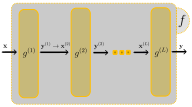
\includegraphics[width=0.9\textwidth]{ch3/assets/raw_net.png}
	\caption{High-level representation of an ANN through function composition showing the dynamics of input $ \x $ all the way to the output $ y $ through $ L $ layers. }
	\label{fig:raw_net}
\end{figure}

\subsubsection{Processing Unit}
Layers contain an array of neurons or processing units (for short, unit). Each unit is capable of accessing the entire length of input features to that layer and it is the element that possesses the parameters of the network (weights and biases). The layer's number of output features is mediated by the number of units present in that layer.

Since each layer has its own sets of units, to keep track of all parameters, we will establish the following definitions:

\begin{itemize}
	\item $ \w{l}{i} $ - weights of neuron $ i $ of layer $ l $. Weights can be a scalar, vector, matrix or generally speaking, a tensor;
	\item $ \bi{l}{i} $ - scalar bias value of neuron $ i $ of layer $ l $;
	\item $ \ints{l} $ - number of input features of layer $ l $;
	\item $ \outs{l} $ - number of units or number of output features of layer $ l $;
	\item $ \intsp{l} $ - input feature shape of layer $ l $;
	\item $ \outsp{l} $ - output feature shape of layer $ l $.
\end{itemize}

Upon receiving the input features, unit $ i $ in layer $ l $ will perform some computation expressed by a function $ \paf{l} $, resulting in one output feature per unit. The quintessential example of such computation is the weighted sum, where if a neuron receives a vector of layer input features $ \x' $,

\begin{equation}
	\pact{l}{i} = \paf{l}(\w{l}{i}, \bi{l}{i}, \x^{(l)}) = \w{l}{i} \cdot \x^{(l)} + \bi{l}{i},
	\label{eq:pact_weighted_sum}
\end{equation}
being $ \paf{l}:  \mathbb{R}^{\ints{l}} \rightarrow \mathbb{R} $, $ \pact{l}{i} $ the pre-activation value of neuron $ i $ of layer $ l $ and "$ \cdot $" denotes the dot product. In this example, $ \pact{l}{i} $ happens to be a scalar\footnote{In general terms, these quantity can also be a tensor depending on the pre-activation operation.} and it was decided to name it pre-activation since the last step of the processing unit computation, is the application of an activation function.

The derivative of the activation function $ \af{l} $ must yield a limited function. This function will receive the pre-activation value from a unit $ i $ of layer $ l $ to filter them to an appropriate range for the network, returning the final output feature or the activation value $ \act{l}{i} $ of the unit,

\begin{equation}
	\act{l}{i} = \af{l}(\pact{l}{i}),
	\label{eq:act}
\end{equation}
where $ \act{l}{i} $ has the same dimensions as $ \pact{l}{i} $. Two standard examples of $ \af{l} $ where $ \af{l}: \mathbb{R} \rightarrow \mathbb{R} $ can be, for instance, the sigmoid function $ \sigma $ or hyperbolic tangent $ \tanh $ operating. The layer $ l $'s output will be a vector of length $ \outs{l} $ containing all $ \act{l}{i} \ \text{for} \ i = 1, 2, ..., \outs{l} $. On a side note, one can see that this process inside a unit is also a composition of functions,

\begin{equation}
	\act{l}{i} = \af{l} \circ \paf{l}(\w{l}{i}, \bi{l}{i}, \x^{(l)})
	\label{eq:comp_act}
\end{equation}

The main gist of a \gls{RVNN} when compared to a \gls{CVNN} is that $ \w{l}{i} \in \mathbb{C}^{\intsp{l}} $ and $ \bi{l}{i} \in \mathbb{C} $ for $ i = 1, 2, ..., \outs{l} $. This small modification on the network's parameters carries out major consequences in the traditional dynamics of \gls{RVNN}.

\subsection{Signal Forwarding}
To forward a signal through an \gls{ANN}, one must define the layers of the network, i.e. defining the functions $ g^{l} $ for $ l = 1, 2, ..., L $ where $ L $ is the number of layers in the network, and calculate the chain composition of functions given input $ \x $ as expressed in equation (\ref{eq:layer_comp_network}). To define the function $ \actf{l} $ where $ \actf{l}: \mathbb{R}^{\intsp{l}} \rightarrow \mathbb{R}^{\outsp{l}} $, one must first understand its action. Since a layer $ l $ will return $ \outs{l} $ output features then,

\begin{multline}
	\y^{(l)} = \actf{l}(\x^{(l)}) = \\ 
	[\af{l} \circ \paf{l}(\w{l}{1}, \bi{l}{1}, \x^{(l)}),
		\af{l} \circ \paf{l}(\w{l}{2}, \bi{l}{2}, \x^{(l)}),
		...,
		\af{l} \circ \ \paf{l} (\w{l}{N}, \bi{l}{N}, \x^{(l)}) ]
\end{multline}
with $ N = \outs{l} $. Indexing the output features yields,

\begin{equation}
	\y^{(l)} = \act{l}{i} = \af{l} \circ \paf{l}(\w{l}{i}, \bi{l}{i}, \x^{(l)}).
\end{equation}
With this in mind, one no longer needs the abstract function $ \actf{l} $. The layer $ l $ can be defined by the pre-activation function $ \paf{l} $ and the activation function $ \af{l} $. It is important to emphasize that, due to abuse of notation, it is not clear that $ \paf{l} $ and $ \af{l} $ can be different functions from $ \paf{l+1} $ and $ \af{l+1} $, which in fact can in cases where the network has multiple layers. If $ L = 1 $ forwarding a signal through the network can be trivial like so,

\begin{equation}
	\y_i =  \act{1}{i} = \af{1} \circ \paf{1} (\w{1}{i}, \bi{1}{i}, \x).
\end{equation}
For a generic $ L $, the entire forward dynamic is summarized as,

\begin{equation}
	\act{l}{i} = \af{l} \circ \paf{l} (\w{l}{i}, \bi{l}{i}, \act{l-1}{j})
\end{equation}
where $ \act{l=0}{i} = \x_i $ being the input to the \gls{ANN} ($ l = 0 $ is a virtual layer) and $ \act{l=L}{i} = \y_i $ the prediction of the network. The generic indices $ i, j $, are used to represent that different layers can have different lengths of input and output features, i.e., typically $ \ints{l} \neq \ints{l-1} $. Additionally, the number of input features of each layer must be equal to the number of output features of the previous layer, i.e. $ \ints{l} = \outs{l-1} $. Figure~\ref{fig:complete_net}, presents an illustrative summary of the notation and dynamics addressed up until this point.

\begin{figure}[htbp]
	\centering
	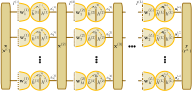
\includegraphics[width=1.0\textwidth]{ch3/assets/complete_net.png}
	\caption{Base architecture of a neural and framing with the formalism introduced in this chapter. In this illustration, $  N = \outs{1} $, $ M = \outs{2}$ and $ K = \outs{L} $. To not make the illustration to dense , the bias parameter was omitted, nevertheless, its framing is analogous to the weights.}
	\label{fig:complete_net}
\end{figure}

\subsection{Complex Activation Functions}
At a high-level, this procedure applies for both \gls{RVNN} and \gls{CVNN}. The major difference happens when one looks at the function $ \paf{l} $ and $ \af{l} $ since now they map values in the complex domain. Proceeding to examining the example of the pre-activation function of the weighted sum in equation (\ref{eq:pact_weighted_sum}) in the complex domain $ \mathbb{C} $. The first instance where this domain offers some non-linearity in the calculations, is in the product between two complex numbers inside the scalar product between $ \w{l}{i} $ and $ \x' = \act{l-1}{j} $.  Considering two complex numbers $ z_1 = x_1 + iy_1 $ and $ z_2 = x_2 + iy_2 $, their multiplication can be expressed in function of each one's real and imaginary components,

\begin{equation}
	z = z_1 z_2 = ( x_1 x_2 - y_1 y_2 ) + i( x_1 y_2 + y_1 x_2 ),
\end{equation}
where $ \Imag{z_1} $ and $\Imag{z_2} $ have an important role in modulating $ \Real{z} $. The second instance is in choosing an activation function for the network.

From this point onward, it is important to start considering the properties of complex numbers and its consequences on a \gls{CVNN}. Since the weights and biases are now complex, even if  the values of the input features carry no imaginary component, the forwarded signal will eventually pick up an imaginary component.

For a function to be viable candidate as an \gls{CAF} $ \af{l}: \mathbb{C}^{\outsp{l}} \rightarrow \mathbb{C}^{\outsp{l}} $ for a given layer $ l $, its derivative needs to have a limited codomain. In the real domain, the previously given examples of $ \sigma $ and $ \tanh $ are actually both limited in its original form and its derivative. However, if we take for instance function $ \sigma $ and provide it a complex argument, it will result in a function that does not have a limited codomain, nor a limited derivative, due to the exponentiation of complex numbers. A typical work around is to define a Real-Imaginary-Type function or Split-Function, as shown in equation (\ref{eq:split_func}).

\begin{equation}
	\af{l}(z) = \af{l}_{r}(\Real{z}) + i \af{l}_{r}(\Imag{z}),
	\label{eq:split_func}
\end{equation}
with $ \af{l}_{r}:  \mathbb{R}^{\outsp{l}} \rightarrow \mathbb{R}^{\outsp{l}} $ a function with limited derivative. Given that $ \af{l}_{r} $ is limited, ensures that  $ \af{l} $ and its derivative is also limited, therefore, a viable candidate as a \gls{CAF}.

A group of split functions can be created based on real-valued \gls{AF} which are present in the library but also two more viable \gls{CAF}. The library also implements the zReLU function

\begin{equation}
	\af{l}(z) = 
	\begin{cases}
		z \ \text{if} \  0 \leqslant \arg(z) \leqslant \frac{\pi}{2} \\
		0 \  \text{otherwise}
	\end{cases},
\end{equation}
Additionally, it also implements an adaptation of the cardioid curve, as a function,

\begin{equation}
	\af{l}(z) = \dfrac{1}{2} ( 1 + \cos(\arg(z)) ) z
\end{equation}
Both functions being explicitly dependent on the phase of $ z $ and with only its derivative as a limited function.

\subsection{Complex Back-Propagation}
In section \ref{subsec:fundamentals} it was defined a set of functions and composition of functions that, at the time, seemed to be just some abstraction. However, these functions will be important for implementing an algorithm based on the gradient descent optimization method \parencite{cauchy1847}, that will make it possible for the \gls{CVNN} to learn through data. This requires knowledge in Complex Analysis, specifically complex function derivatives, and using the complex chain rule in the composition of functions to implement Complex Back-Propagation \parencite{rumelhart1986}.

Before going through complex differentiation, let us quickly define a complex loss function. Although a simple concept, it is crucial for implementing complex gradient descent (or optimization algorithms in general).

Typically, in the real domain, one can define the \gls{RVNN} loss function as,

\begin{equation}
	\loss_n = \left( \act{L}{n} - r_n \right)^2,
	\label{eq:error_cp}
\end{equation}
where $ \loss_n $ represents the error of neuron $ n $ given last layer's activation $ \act{L}{n} $ and $ r_n $ the target output feature result (from the dataset). A mean or a sum can be performed along the flatten values of $ \loss_n $ for instance to a single value of the loss function expressed in equation (\ref{eq:losstotal}) 

\begin{equation}
	\loss = \sum_{n}^{\outs{L}} \loss_n,
	\label{eq:losstotal}
\end{equation}

In the complex domain, not a lot changes in the error expression $ \loss_n: \mathbb{C}^{\outsp{L}} \rightarrow \mathbb{R}^{\outsp{L}} $, since a complex codomain is not going to be considered. The complex error function can be,

\begin{equation}
	\loss_n = \left| \act{L}{n} - r_n \right|^2,
	\label{eq:cerror}
\end{equation}
with $ \left| \act{L}{n} - r_n \right| $ being the absolute value of the complex number resultant from $ \act{L}{n} - r_n $.

\subsubsection{Complex differentiation}
Differentiating a complex function is going to be the most important task to perform in the complex gradient descent (as a consequence, complex back-propagation), and it is important to recognize certain types of complex functions.

In complex analysis, an Holomorphic function is a function that obeys the Cauchy-Riemann equations \parencite{Cauchy1814}. Given a function $ f(z) = u(x,y) + iv(x,y) $ where $ z = x + iy $, the Cauchy-Riemann equations read,

\begin{equation}
	\der{u}{x} = \der{v}{y}, \ \der{u}{y} = -\der{v}{x}.
	\label{eq:cr}
\end{equation}
If such a function $ f $ obeys these equations, then its derivative with respect to $ z $ can be easily taken according to,

\begin{equation}
	\der{f}{z} = \der{u}{x} + i\der{v}{x}.
	\label{eq:cr_der}
\end{equation}
However, in this scenario of \gls{CVNN}, functions typically do not obey equations in (\ref{eq:cr}). These functions are called non-holomorphic, and equation in (\ref{eq:cr_der}) no longer holds true. To compute the derivative of a non-holomorphic function, one must first layout the chain rule between a complex function and its argument's real and imaginary part like so,

\begin{equation}
	\begin{cases}
		\der{f}{z} = \der{f}{x}\der{x}{z} + \der{f}{y}\der{y}{z} \\
		\\
		\der{f}{\conj{z}} = \der{f}{x}\der{x}{\conj{z}} + \der{f}{y}\der{y}{\conj{z}}
	\end{cases},
	\label{eq:complex_chain_der}
\end{equation}
being $ \conj{z} $ the complex conjugate of $ z $. Here, we are considering also the derivative with respect to $ \conj{z} $ because both $ x $ and $ y $, have an implicit dependence in $ z $ and $ \conj{z} $ as show in equation (\ref{eq:xydepz}),

\begin{equation}
	\begin{cases}
		x = \dfrac{z + \conj{z}}{2} \\
		\\
		y = \dfrac{z - \conj{z}}{2i}
	\end{cases}.
	\label{eq:xydepz}
\end{equation}
We can use this dependency to simplify equation in (\ref{eq:complex_chain_der}) yielding,
\begin{equation}
	\begin{cases}
		\der{f}{z} = \dfrac{1}{2} \left( \der{f}{x} - i\der{f}{y} \right) \\
		\\
		\der{f}{\conj{z}} = \dfrac{1}{2} \left( \der{f}{x} + i\der{f}{y} \right)
	\end{cases}.
	\label{eq:complex_chain_der_simp}
\end{equation}
These derivative expressions are valid for both holomorphic and non-holomorphic functions, however, one would see that the second is null for the holomorphic case. This is an important fact since, computationally-wise, if one knows from the start that a function is holomorphic: calculating its conjugate derivative is not necessary; a more straight-forward expression can be taken; last but not least, no need for storing unnecessary null data regarding the conjugate derivative and perform further calculations with just zeros.

The function definitions established in Section \ref{subsec:fundamentals}, will help categorize each one to simplify the back-propagation algorithm as much as possible.

\subsubsection{Holomorphic \& Non-Holomorphic functions in a \gls{CVNN}}
\label{subsubsec:holo_non_holo}
\paragraph{Pre-Activation Function $ \paf{l} $} 
The most common example of a $ \paf{l} $, is the (complex) weighted sum showed in equation (\ref{eq:pact_weighted_sum}), which for the sake of this library, only layer logics based on the weighted sum will be used (common weighted sum and convolution). First point is to know if such function is holomorphic, therefore, one needs to apply the Cauchy Riemann equations in \ref{eq:cr}. If it proves that the complex summation function $ f_1(z) = z + z_0 $ and the complex multiplication function $ f_2(z) = z z_0 $ are holomorphic, due to the properties of holomorphic functions \parencite{wirtinger1927formalen}, we can prove that the sum of complex products, is holomorphic (which is what a weighted sum is). For $ f_1 $ there is,

\begin{equation}
	\begin{cases}
		u(x,y) = x + x_0 \Rightarrow \der{u}{x} = 1, \ \der{u}{y} = 0 \\
		\\
		v(x,y) = y + y_0 \Rightarrow \der{v}{x} = 0, \ \der{v}{y} = 1
	\end{cases},
	\label{eq:cauchypactholo}
\end{equation}
with $ z_0 = x_0 + iy_0 $. Equation (\ref{eq:cauchypactholo}) shows that the summation function is holomorphic. For $ f_2 $,

\begin{equation}
	\begin{cases}
		u(x,y) = x  x_0 - y y_0 \Rightarrow \der{u}{x} = x_0, \ \der{u}{y} = -y_0 \\
		\\
		v(x,y) = x y_0 + y x_0 \Rightarrow \der{v}{x} = y_0, \ \der{v}{y} = x_0
	\end{cases},
\end{equation}
where Cauchy-Riemann Equations also hold. Therefore yields,

\begin{equation}
	\paf{l}(\w{l}{i}, \bi{l}{i}, \act{l-1}{j}) = \w{l}{i} \cdot \act{l-1}{j} + \bi{l}{i}, \  \forall\w{l}{i}, \act{l-1}{j}, \bi{l}{i} \in \mathbb{C},
\end{equation}
being an holomorphic function. According to equation (\ref{eq:cr_der}), one can determine what are going to be the relevant partial derivatives for the back-propagation algorithm in equation (\ref{eq:reldel}),

\begin{equation}
	\begin{cases}
		\der{\paf{l}}{\act{l-1}{j}} = \w{l}{i} \\
		\\
		\der{\paf{l}}{\w{l}{i}} = \act{l-1}{j} \\
		\\
		\der{\paf{l}}{\bi{l}{i}} = 1 \\
		\\
		\left( \der{\paf{l}}{\cact{l-1}{j}} = \der{\paf{l}}{\cw{l}{i}} = \der{\paf{l}}{\cbi{l}{i}} = 0 \right)
	\end{cases}.
	\label{eq:reldel}
\end{equation}

\paragraph{Complex Activation Functions $ \af{l} $}
Considering the set of activation functions present in this library, all happen to be non-holomorphic with the exeption of zReLU. By reviewing the split-function in equation (\ref{eq:split_func}), one proves that all split-functions are non-holomorphic, by applying the Cauchy-Riemann Equation in equation (\ref{eq:creq_split}),

\begin{equation}
	\begin{cases}
		u(x,y) = u(x) = \af{l}_r(\Real{z}) \Rightarrow \der{u}{x} = \der{\af{l}_r}{x}, \ \der{u}{y} = 0 \\
		\\
		v(x,y) = v(y) = \af{l}_r(\Imag{z}) \Rightarrow \der{v}{x} = 0, \ \der{v}{y} = \der{\af{l}_r}{y}
	\end{cases}.
	\label{eq:creq_split}
\end{equation}
Given the explicit dependency of $ u = u(x) $ and $ v = v(y) $, its derivatives with respect to $ x $ and $ y $ respectively, are always going to be different aside from when $ x = y $. Nevertheless, since the entire domain of the split-functions is used, differentiation is performed with equation
(\ref{eq:complex_chain_der_simp}) resulting in,

\begin{equation}
	\begin{cases}
		\der{\af{l}}{z} = \dfrac{1}{2} \left( \der{\af{l}_r}{x} + \der{\af{l}_r}{y} \right) \\
		\\
		\der{\af{l}}{\conj{z}} = \dfrac{1}{2} \left( \der{\af{l}_r}{x} - \der{\af{l}_r}{y} \right)
	\end{cases}.
\end{equation}

\paragraph{Complex Loss Function $ \af{l} $}
Differentiating the complex error function in equation (\ref{eq:cerror}) is the starting point to determine the entire gradients of the network, since it is going to dictate what is the downward direction to optimize the error for each neuron, and as a consequence, downward direction in the entire loss function surface.

First checking if the error function in equation (\ref{eq:cerror}), is holomorphic, and for simplicity, considering $ \norm{\act{L}{n} - r_n}^2 = \norm{z}^2 = x^2 + y^2 $,

\begin{equation}
	\begin{cases}
		u(x,y) =  = x^2 + y^2 \Rightarrow \der{u}{x} = 2x, \ \der{u}{y} = 2y \\
		\\
		v(x,y) = 0 \Rightarrow \der{v}{x} = 0, \ \der{v}{y} = 0
	\end{cases}.
\end{equation}
So this tells that the complex absolute value function is a non-holomorphic function, therefore, the loss function is only holomorphic for error values of zero (which is going to be never a reachable value). One needs to consider the non-holomorphic derivatives, which after some basic algebra yields,

\begin{equation}
	\begin{cases}
		\der{\loss_n}{\act{L}{n}} = \cact{L}{n} - \conj{r}_n \\
		\\
		\der{\loss_n}{\cact{L}{n}} = \act{L}{n} - r_n
	\end{cases}.
\end{equation}

\subsubsection{Complex Chain Rule}
To implement an optimization method based on the complex gradient descent, only rests to define a chain rule for propagating derivatives. 

Supposing two generic complex functions $ A $ and $ B $ have a dependency in $ z $ and in $ \conj{z} $ in case $ A $ and $ B $ are non.holomorphic. If there is a complex function $ C = B \circ A $, then to compute the chain rule, one must consider $ z $ and $ \conj{z} $. So, the chain rule for $ B \circ A $ where both functions are non-holomorphic is,

\begin{equation}
	\begin{cases}
		\der{(B \circ A)}{z} = \der{B}{A}\der{A}{z} + \der{B}{\conj{A}}\der{\conj{A}}{z} \\
		\\
		\der{(B \circ A)}{\conj{z}} = \der{B}{A}\der{A}{\conj{z}} + \der{B}{\conj{A}}\der{\conj{A}}{\conj{z}} \\
	\end{cases}
	\label{eq:AB_nonholo}
\end{equation}
where properties such as,

\begin{equation}
	\begin{cases}
		\der{\conj{A}}{z} = \text{conj}\group{\der{A}{\conj{z}}} \\
		\\
		\der{\conj{A}}{\conj{z}} = \text{conj}\group{\der{A}{z}}
	\end{cases},
	\label{eq:comp_conj_div}
\end{equation}
hold for these derivatives where, for readability, $ \text{conj}(z) = \conj{z} $. However, if $ A $ is holomorphic,

\begin{equation}
	\begin{cases}
		\der{(B \circ A)}{z} = \der{B}{A}\der{A}{z} \\
		\\
		\der{(B \circ A)}{\conj{z}} = \der{B}{\conj{A}}\der{\conj{A}}{\conj{z}} \\
	\end{cases},
\end{equation}
else if $ B $ is holomorphic,
\begin{equation}
	\begin{cases}
		\der{(B \circ A)}{z} = \der{B}{A}\der{A}{z} \\
		\\
		\der{(B \circ A)}{\conj{z}} = \der{B}{A}\der{A}{\conj{z}} \\
	\end{cases},
	\label{eq:B_holo}
\end{equation}
else if $ A $ and $ B $ are both holomorphic,

\begin{equation}
	\begin{cases}
		\der{(B \circ A)}{z} = \der{B}{A}\der{A}{z} \\
		\\
		\der{(B \circ A)}{\conj{z}} = 0 \\
	\end{cases}.
\end{equation}
These expressions are very much important in the Complex Back-Propagation algorithm as it will become apparent.

\subsubsection{Complex Gradient Descent \& Back-Propagation}
In the task of optimizing a neural network based on the gradient descent optimization method, the objective is to determine the gradient of the loss function like so,

\begin{equation}
	\begin{cases}
		\der{\loss}{\w{l}{i}}  = \der{\group{\loss \circ f}}{\w{l}{i}} = 
		\der{\group{\loss \circ \group{g^{(L)} \circ ... \circ g^{(2)} \circ g^{(1)}}}}{\w{l}{i}} \\
		\\
		\der{\loss}{\bi{l}{i}}  = \der{\group{\loss \circ f}}{\bi{l}{i}} = 
		\der{\group{\loss \circ \group{g^{(L)} \circ ... \circ g^{(2)} \circ g^{(1)}}}}{\bi{l}{i}} \\
	\end{cases},
\end{equation}
since $ g^{l} = \af{l} \circ \paf{l} $ and the only adjustable parameters of the network are $ \w{l}{i} $ and $ \bi{l}{i} $ for every $ l = 1, 2, ..., L $ and $ i = 1, 2, ..., \ints{l} $\footnote{The index $ i $ is implicitly dependent on $ l $}.

This derivative is not straightforward to determine, because the only starting point is from the loss function it to optimize it with an explicit dependence on only last layer's activation $ \act{L}{n} $. The way one determines the full derivative is by applying the back-propagation algorithm.

First, the loss function's dependency with respect to last layer's weights and biases, $ \w{L}{n} $ and $ \bi{L}{n} $ respectively is,

\begin{equation}
	\begin{cases}
		\der{\loss}{\w{L}{n}} = \der{\group{\loss \circ \act{L}{n}}}{\w{L}{n}} \\
		\\
		 \der{\loss}{\bi{L}{n}} = \der{\group{\loss \circ \act{L}{n}}}{\bi{L}{n}}
	\end{cases}.
\end{equation}
Because of the properties mentioned in equation (\ref{eq:comp_conj_div}) and the fact that $ \func[\loss]{\set{C}^{\outsp{L} \otimes \outs{L}}}{\set{R}} $ results in,

\begin{equation}
	\begin{cases}
		\der{\loss}{\cw{l}{i}} = \text{conj}\group{\der{\loss}{\w{l}{i}}} \\
		\\
		\der{\loss}{\cbi{l}{i}} = \text{conj}\group{\der{\loss}{\bi{l}{i}}}
	\end{cases}.
\end{equation}

Going back to section~\ref{subsubsec:holo_non_holo}, $ \act{L}{n} $  as function of $ \pact{L}{n} $, is a non-holomorphic function just like $ \loss(\act{L}{n})  $. Therefore, one can use equation in (\ref{eq:AB_nonholo}) to determine the derivative compositions,

\begin{equation}
	\begin{cases}
		\der{\loss}{\w{L}{n}} = \der{\loss}{\act{L}{n}}\der{\group{\act{L}{n} \circ \pact{L}{n}}}{\w{L}{n}} + \der{\loss}{\cact{L}{n}}\der{\group{\cact{L}{n} \circ \pact{L}{n}}}{\w{L}{n}} \\
		\\
		\der{\loss}{\bi{L}{n}} = \der{\loss}{\act{L}{n}}\der{\group{\act{L}{n} \circ \pact{L}{n}}}{\bi{L}{n}} + 	\der{\loss}{\cact{L}{n}}\der{\group{\cact{L}{n} \circ \pact{L}{n}}}{\bi{L}{n}} 
	\end{cases}.
\end{equation}
Nevertheless, $ \act{L}{n}(\pact{L}{n}) $ (result of function $ \paf{L} $) does not have an explicit dependency in $ \w{L}{n} $ but $ \pact{L}{n}(\w{L}{n}, \bi{L}{n}, \act{L-1}{m}) $ has (result of function $ \af{L} $). As  shown in section~\ref{subsubsec:holo_non_holo} that $ \pact{L}{n} $ is holomorphic so it is possible to apply equation in (\ref{eq:B_holo}). Establishing the following definitions in equation (\ref{eq:lossdef}) beforehand to make the equations more readable,

\begin{equation}
	\begin{cases}
		\ploss{L}{n} \equiv \der{\loss}{\act{L}{n}}\der{\act{L}{n}}{\pact{L}{n}} \\
		\\
		\pcloss{L}{n} \equiv \der{\loss}{\cact{L}{n}}\der{\cact{L}{n}}{\pact{L}{n}} \\
	\end{cases}.
	\label{eq:lossdef}
\end{equation}
The derivative of the loss function with respect to the weights and biases of the last layer is,

\begin{equation}
	\begin{cases}
		\der{\loss}{\w{L}{n}} = \group{\ploss{L}{n}+ \pcloss{L}{n}}\der{\pact{L}{n}}{\w{L}{n}} \\
		\\
		\der{\loss}{\bi{L}{n}} = \group{\ploss{L}{n} + \pcloss{L}{n}}\der{\pact{L}{n}}{\bi{L}{n}} \\
	\end{cases}.
\end{equation}

Now the next step is to determine the derivative of the loss function with respect to the weights and biases of the previous to last layer represented in equation (\ref{eq:prev_layer_wb}),

\begin{equation}
	\begin{cases}
		\der{\loss}{\w{L-1}{m}} = \group{\ploss{L-1}{m} + \pcloss{L-1}{m}}\der{\pact{L-1}{m}}{\w{L-1}{m}} \\
		\\
		\der{\loss}{\bi{L-1}{m}} = \group{\ploss{L-1}{m} + \pcloss{L-1}{m}}\der{\pact{L-1}{m}}{\bi{L-1}{m}} \\
	\end{cases},
	\label{eq:prev_layer_wb}
\end{equation}
where in this expression,  all values are known aside from $ \ploss{L-1}{m} $ and $ \pcloss{L-1}{m} $.

The key to the back-propagation algorithm, is determining the derivative of the loss function with respect to the previous to last layer's activation such that one can keep iterating backwards until the input layer ($ l = 1 $) is reached. Therefore yields,

\begin{equation}
	\der{\loss}{\act{L-1}{m}} = \sum_{n} \left[ \group{\ploss{L}{n} + \pcloss{L}{n}}\der{\pact{L}{n}}{\act{L-1}{m}} \right],
	\
	\der{\loss}{\cact{L-1}{m}} =  \text{conj}\group{\der{\loss}{\act{L-1}{m}}} \\
	\label{eq:back_prop}
\end{equation}
where the sum over the units $ n $, means that each neuron $ m $ of layer $ L-1 $ contributes equally to every neuron's activation of layer $ L $.

Now one can use equation in (\ref{eq:back_prop}) to determine the values of $ \ploss{L-1}{m} $ and $ \pcloss{L-1}{m} $ and insert them in equation (\ref{eq:prev_layer_wb}) to propagate the derivatives backwards.

This Complex Back-Propagation is implemented by the proposed library and a summary can be visualized in Figure~\ref{fig:backprop}. In upcoming sections, some small technical details regarding the implementation of this algorithm will be discussed and some other operations relevant to \gls{CVNN} modeling.

\begin{figure}[htbp]
	\centering
	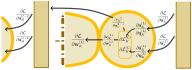
\includegraphics[width=1.0\textwidth]{ch3/assets/cp_backprop.png}
	\caption{Depiction summarizing the complex back-propagation algorithm, at the neuron level, used in Renplex. Arrows indicate calculations and one can see that, computational-wise, the majority of the derivatives can be calculated in parallel. Derivatives related to the bias were omitted for a more concise illustration and here $ M = \outs{L-1} $ and $ K = \outs{L} $}.
	\label{fig:backprop}
\end{figure}

\section{Structure of the Library}

The library is structured in 8 modules:

\begin{itemize}
	\item \texttt{act} : Activation function definitions and interface for computing activation values;
	\item \texttt{cvnn}: Core module that contains structures and tools for modulating \gls{CVNN} architectures.
	\item \texttt{dataset}: Interface for processing datasets automatically;
	\item \texttt{err}: Minimal error handling enumerations;
	\item \texttt{init}: Enumerations for computing layer initialization techniques;
	\item \texttt{input}: Enumerations for handling static input and output features shapes for layers;
	\item \texttt{math}: Various mathematical utilities concerning, for instance, complex float, matrix definition and operations and random number generation;
	\item \texttt{opt}: Definition and computing loss function and its derivatives.
\end{itemize}

A brief overview on the core module \texttt{cvnn}.

\paragraph{\texttt{cvnn} Module}
The core module \texttt{cvnn}, only possesses two additional modules: \texttt{layer} and \texttt{network}. \texttt{layer} module is arguably the most important as it contains all the layers implemented in the library each one with its own logic, being:

\begin{itemize}
	\item \texttt{DenseCLayer}: Contains a matrix of weights, vector of biases (as many as there is units), and an activation function. It represents a fully connected layer that performs the common weighted sum in equation (\ref{eq:pact_weighted_sum}) given a vector of scalar input features;
	\item \texttt{Flatten}: Flattens out a vector of matrix input features into a vector of scalar input features;
	\item \texttt{ConvCLayer}: Contains a matrix of weights (filters/kernels), a vector of biases and an activation function. This layer computes the convolution between every matrix input feature against every filter. The number of filters will dictate the number of output features (matrices);
	\item \texttt{Reduce}: A generalized pooling operation that asks for the user the operation to be applied on each block of each input feature matrix. Each matrix block of every input feature will be reduced into a scalar for down-sampling data.
\end{itemize}

The \texttt{network} module only defines the \texttt{struct} of a network, being a vector of layers, and underlying operations such as running the complex gradient descent optimization for a batch of data, adjusting the weights of the layers accordingly, calculating loss and accuracy, and forwarding and intercepting signals.

Having this quick layout of the library, the main implemented features, operations and critical algorithms will be addressed.

More details on the structure of the library can be viewed in the Github repository \href{https://github.com/Pxdr0-A/renplex.git}{Pxdr0-A/renplex.git}, it is also published in the crates.io, the official package manager for Rust in \href{https://crates.io/crates/renplex}{https://crates.io/crates/renplex}. Documentation for this library can also be accessed in \href{https://docs.rs/renplex/0.1.1/renplex/}{https://docs.rs/renplex/0.1.1/renplex/}.

\section{Main Implementations}
To give some insights on the operation and performance of the library, in this section, there will be an overview on the most critical tasks executed in the library.

\subsection{Matrix-Vector Multiplication}

The Rust implementation for this operations goes as follows:

\begin{lstlisting}[caption=Onverview on the Matrix-Vector multiplication implemented in the Renplex Library using Rust.]
	pub fn mul_slice(
		&self, 
		rhs: &[T]
	) -> Result<Vec<T>, OperationError> {
		
		// error handling
		...
		
		// map rows of the matrix
		let res = self.rows_as_iter().map(|elm| {
			// create a row and vec iterator
			elm.into_iter()
			.zip(rhs.iter())
			// perform scalar product
			.fold(T::default(), |acc, elm| { 
				acc + (*elm.0 * *elm.1) 
			})
		}).collect::<Vec<_>>();
		
		Ok(res)
	}
\end{lstlisting}

Here, the slice \texttt{rhs:\&[T]}  is representing a vector and \texttt{\&self} is a reference in memory to a matrix. Afterwards, rows of the matrix are taken and mapped to a folded value that represents the (complex) scalar product between matrix row and vector. The collection of these folded values forms the result vector.

The majority of these algorithms were built with some flexibility in case there is need for parallelization or eventual GPU utilization. This algorithm is easy to add concurrency  in the aspect that each folded value resultant from scalar matrix row and vector, can be computed independently.

\subsection{2D Convolution}
\label{sec:2Dconv}

As for the 2D convolution, the high-level layout of the algorithm used can be viewed in Listing~\ref{lst:convprod}.

\begin{lstlisting}[label=lst:convprod,caption=Overview on the Convolutional Product implemented in the Renplex library using Rust.]
	pub fn convolution(
		&self, 
		kernel: &Self
	) -> Result<Self, OperationError> {
		
		// extract kernel and matrix shape
		let k_shape = kernel.get_shape();
		let initial_shape = self.get_shape();
		
		// error handling
		...
		
		// determine the final shape
		let final_shape = [
			initial_shape[0] - (k_shape[0]-1), 
			initial_shape[1] - (k_shape[1]-1)
		];
		
		// go through the number of final rows
		let convolved_body = (0..final_shape[0])
			.into_iter()
			.flat_map(|i| {
				// get a retangular matrix to slide the kernel
				let slider = self.get_slider(i, k_shape[0]);
				
				// slide the kernel
				let conv_row = slider.slide(&kernel)
				
				// returns a convolved row
				conv_row
		}).collect::<Vec<_>>();
		
		// convert a flatten matrix to the final shape
		Ok(convolved_body.to_matrix(final_shape).unwrap())
	}
\end{lstlisting}

The way this convolution is going to be performed is by calculating the convolution per rows of the final shape. This is, it is going to get a "slider" from the matrix which is requesting as many rows as there are rows in the kernel\footnote{For example, if the kernel shape is $ 3\times 4 $ it will request $ 3 $ rows.} and make the kernel slide through it to compute the scalar product per block. This yields a convolved row that will collected into a vector later converted to a matrix as the result.

Such implementation guarantees also an easy parallelization if one wishes to compute convolved rows concurrently by getting a reference to a slider of the matrix in whatever thread needed.

Some examples of convolutions performed by this algorithm can be found in Figure~\ref{fig:4conv}, with an example of a handwritten 4 in the MNIST dataset \parencite{lecun1998mnist}.

\begin{figure}[htbp]
	\centering
	\subfigure[]{
		\includegraphics[width=0.3\textwidth]{ch3/assets/4.png}
		\label{fig:4original}
	}
	\subfigure[]{
		\includegraphics[width=0.3\textwidth]{ch3/assets/4_sharpen.png}
		\label{fig:4sharpen}
	}
	\subfigure[]{
		\includegraphics[width=0.3\textwidth]{ch3/assets/4_sobel.png}
		\label{fig:4sobel}
	}
	\caption{A handwritten "4" of the MNIST dataset in (a), and the results for the applications of two different convolutional filters using the Renplex library. In (b), the application of a $ 3 \times 3 $ shapen filter and in (c) the application of the sobel operator \parencite{sobel2014operator}.}
	\label{fig:4conv}
\end{figure}

In this three Figures we have in \ref{fig:4original} the original image, in \ref{fig:4sharpen} the application of the sharpen filter,

\[
\begin{pmatrix}
	0.0 & -1.0 & 0.0 \\
	-1.0 & 5.0 & -1.0 \\
	0.0 & -1.0 & 0.0 \\
\end{pmatrix},
\]

and in \ref{fig:4sobel} the application of the Sobel Operator \parencite{sobel1968}, both filters with a size of $ 3 \times 3 $. 

In both of these procedure there is the downsize of the image because the convolution is reducing a $ 3 \times 3 $ block to $ 1 $ value, thus effectively reducing dimension by $ 2 $ rows and $ 2 $ columns, in this case.

\subsection{2D Down-Sampling \& Up-Sampling}

A crucial set of operations involved in convolutional neural networks is the and down-sampling up-sampling.

\paragraph{Down-Sampling}
For the down-sampling it was used a general pooling operation similar to the \href{https://scikit-image.org/docs/stable/api/skimage.measure.html#skimage.measure.block_reduce}{\texttt{skimage.measure.block\_reduce}} function present in the scikit-image \parencite{van2014scikit} python library, it divides the matrix in blocks and reduces them to single values based on a certain function. This can be viewed on Listing~\ref{lst:reduceop}.

\begin{lstlisting}[label=lst:reduceop,caption=Overview on the Reduce operation on images implemented in the Renplex library using Rust.]
	pub fn block_reduce(
		&self, 
		block_size: &[usize], 
		block_func: impl Fn(&[T]) -> T
	) -> Result<Self, OperationError> {
		
		let matrix_shape = self.get_shape();
		
		// error handling
		...
		
		// determine the final shape
		let final_shape = [
			matrix_shape[0] / block_size[0];
			matrix_shape[1] / block_size[1];
		];
		
		// go through the number of final rows
		let reduced_body = (0..final_shape[0])
			.into_iter()
			.flat_map(|i| {
				// get a retangular matrix to slide the kernel
				let slider = self.get_slider(i, block_size[0]);
			
				// reduce the slider per block 
				// (stride of block_size[1])
				let reduced_row = slider
					.reduce(block_size, block_func)
			
				// returns the reduced slider
				reduced_row
		}).collect::<Vec<_>>();
		
		// convert a flatten matrix to the final shape
		Ok(reduced_body.to_matrix(final_shape).unwrap())
	}
\end{lstlisting}

It is very similar to the 2D convolution, however it adds a stride of \texttt{block\_size[1]} and a custom operation on the block aside from weighted sum (scalar product). Concurrency can be used in the same way as the convolution.

\paragraph{Up-Sampling}

This library only implements on up-sampling technique which is fractional up-sampling and it is used here to propagate the derivatives through a reduce layer. Such technique, receives a block shape saying how much one wants to increase the size of the image by padding in between pixel values (let us call it inner padding), and a kernel that performs a padded convolution after this inner padding is performed. This implementation is slightly bigger than the above ones mentioned so we are just going to show a high-level implementation on Listing~\ref{lst:fracup}.

\begin{lstlisting}[label=lst:fracup,caption=Overview on the Fractional Up-sampling implementation in the Renplex library using Rust.]
	pub fn fractional_upsampling(
		&self, 
		block_size: &[usize], 
		kernel: &Self
	) -> Result<Matrix<T>, OperationError> {
		
		let matrix_shape = self.get_shape();
		let mut matrix_rows = self.rows_as_iter();
		
		// error handling
		...
		
		// appropriate padding size wrapping pixles
		let inner_pad = calc_inner_pad(block_size);
		
		let final_shape = [
			matrix_shape[0] * block_size[0], 
			matrix_shape[1] * block_size[1]
		];
		
		let mut res = Vec::new();
		let n_rows = matrix_shape[0];
		// add inner paddings to the entire image
		// go through all pixels in the image
		for _ in 0..n_rows {
			// add upper padding
			for _ in 0..inner_pad[0] {
				// add as many rows as upper paddings
				res.extend(vec![T::default(); final_shape[1]]);
			}
			// add row with padding in between
			for row_elm in matrix_rows.next().unwrap() {
				// left inner pad
				res.extend(vec![T::default(); inner_pad[1]]);
				res.push(*row_elm);
				// right inner pad
				res.extend(vec![T::default(); inner_pad[2]]);
			}
			// add lower padding
			for _ in 0..inner_pad[3] {
				// add as many rows as lower paddings
				res.extend(vec![T::default(); final_shape[1]]);
			}
		}
		
		// create a result matrix
		let matrix_res = Matrix::from_body(
			res, 
			[final_shape[0], final_shape[1]]
		);
		let kernel_shape  = kernel.get_shape();
		
		// perform padded convolution so that 
		// dimensionality is not lost
		// and values are added in between
		let out = matrix_res
			// by default the filter should be [3, 3]
			.pad((kernel_shape[0]-2, kernel_shape[0]-2))
			.convolution(kernel)
			.unwrap();
		
		Ok(out)
	}
\end{lstlisting}

Typically the kernel used in fractional up-sampling is,

\[
\begin{pmatrix}
	0.25 & 0.50 & 0.25 \\
	0.50 & 1.00 & 0.50 \\
	0.25 & 0.50 & 0.25 \\
\end{pmatrix},
\]
where, to up-sample both real and imaginary parts equally in a complex image, this kernel has to be composed of real values.

On Figure~\ref{fig:4pool} we give an example of an average pooling being performed, and reverting back to the original dimensions with fractional up-sampling of an image with real pixels. Process reads from \ref{fig:4original_pool} to \ref{fig:4fracup}.

\begin{figure}[htbp]
	\centering
	\subfigure[]{
		\includegraphics[width=0.3\textwidth]{ch3/assets/4.png}
		\label{fig:4original_pool}
	}
	\subfigure[]{
		\includegraphics[width=0.3\textwidth]{ch3/assets/4_pool.png}
		\label{fig:4avgpool}
	}
	\subfigure[]{
		\includegraphics[width=0.3\textwidth]{ch3/assets/4_pool_up.png}
		\label{fig:4fracup}
	}
	\caption{A handwritten "4" of the MNIST dataset in (a), and the results for the applications of average pooling (b) and fractional up-sampling (c) in succession using the Renplex library}
	\label{fig:4pool}
\end{figure}


\subsection{Layer Initialization}

Various methods for layer initialization were implemented in this library but they circle around a core method of generating complex numbers. When generating random complex numbers, this library generates a random number between 0 and a certain value defined by the user. This value is going to be the absolute value of the complex number, then it generates a random phase between $  (0, 2\pi) $. The complex number is then converted to real and imaginary part.

In spite of initialization methods like He Initialization \parencite{he2015delving}, Xavier, Xavier Glorot (uniform and normal distribution) \parencite{glorot2010understanding} being used in RVNN, an adaptation of this methods were implemented. Each initialization method's distribution targets the absolute value of the complex number and the phase is again generated according to a uniform distribution.

Listing~\ref{lst:gen} shows how to generate two random complex numbers with this adapted versions Xavier Glorot (Uniform) and He initialization.

\begin{lstlisting}[label=lst:gen,caption=Demonstration of how to generate complex random numbers with Xavier Glorot Uniform and He initialization respectively.]
	use renplex::init::InitMethod;
	
	let ref mut seed: &mut u128 = 63478262957;
	
	// number of input features of a certain layer
	let ni: usize = 64;
	// number of output features of a certain layer
	let no: usize = 16;
	
	// value generated according to Xavier Glorot Uniform
	let xav_glo_num = InitMethod::XavierGlorotU(ni + no)
		.gen(seed);
	
	// value generated according to He Initialization
	let he_init_num = InitMethod::HeInit(ni)
		.gen(seed);
\end{lstlisting}
since each one of these methods his based of on either $ \ints{l} $,  $ \outs{l} $ or both.

\subsection{Complex Back-Propagation}

Initially, two pipelines for the complex back-propagation were tested. The current implemented pipeline can be viewed in Listing~\ref{lst:backprop}.

\begin{lstlisting}[label=lst:backprop, caption=Overview of the gradient optimization algorithm (using back-propagation) implementation in the Renplex library  using Rust., label=lst:grad_opt]
	pub fn gradient_opt(
		&mut self, 
		data: Dataset<T, T>, 
		loss_func: &ComplexLossFunc, 
		lr: T
	) -> Result<(), ForwardError> {
		
		let n_layers = self.layers.len();
		
		// error handling
		...
		
		// weights and biases bgradients to accumulate
		let mut dldw_per_layer = Vec::new();
		let mut dldb_per_layer = Vec::new();
		let mut _total_params: usize = 0;
		
		// allocation of memory for the gradients
		// ...
		
		// make an iterator of the data points 
		let (inputs, targets) = data.points_into_iter();
		
		let batch_size = inputs.len();
		for (input, target) in inputs.zip(targets) {
			// collect all activations of the network
			let mut activations = self
				.collect_acts(input)
				.unwrap()
				.into_iter()
				.rev();
			
			// initial prediction
			let initial_pred = activations.next().unwrap();
			// initial value of loss derivatives
			let mut dlda = T::d_loss(
				initial_pred,
				target,
				&loss_func
			).unwrap().to_vec();
			// initial conjugate derivative of loss
			let mut dlda_conj: Vec<T> = dlda
				.iter()
				.map(|elm| { elm.conj() })
				.collect();
			
			// reversed layers iterator
			let rev_l = self.layers.iter().rev();
			// layers and activations reversed iterator
			let act_l_rev = activations.zip(rev_l).enumerate();
			// activations are consumed here recursively
			for (l, (prev_act, layer)) in act_l_rev {
				// check if layer propagates derivatives
				if layer.propagates() {
					let dldw; let dldb;
					// compute derivatives of the layer l
					// loss and conj loss derivative are being updated
					(dldw, dldb, dlda, dlda_conj) = layer
						.comp_grad(&prev_act, dlda, dlda_conj)
						.unwrap();
					
					// update gradients of the batch
					dldw_per_layer[n_layers-l-1].add_slice_mut(&dldw)
						.unwrap();
					dldb_per_layer[n_layers-l-1].add_slice_mut(&dldb)
						.unwrap(); 
				}
			}	
			// drop unecessary memory
			drop(dlda); drop(dlda_conj);
		}	
		// divide the gradient by the count of data samples
		let scale_param = lr / T::usize_to_complex(batch_size);
		
		// iterator containing the gradients per layer
		let update_iter = dldw_per_layer
			.into_iter()
			.zip(dldb_per_layer.into_iter())
			.zip(self.layers.iter_mut());
		
		update_iter.for_each(|((mut dldw, mut dldb), layer)| {
			if layer.propagates() {
				// scale the gradients
				dldw.mul_mut_scalar(scale_param).unwrap();
				dldb.mul_mut_scalar(scale_param).unwrap();
				// adjust the weights and biases of that layer
				layer.neg_conj_adjustment(dldw, dldb).unwrap();
			}
		});
		
		Ok(())
	}
\end{lstlisting}
Where in Listing~\ref{lst:backprop}, \texttt{self} now is a network \texttt{struct}/instance. This gradient optimization, for each data point in the batch, collects all activations of the network, reverses them, and starts clearing this features as they are needed for the derivative computation of each layer. After accumulating all of the calculated derivatives, it averages them out and multiplies by the learning rate and uses the result to adjust the weights and biases of each respective layer.

The alternative approach (not shown here as a listing), consumes much less memory, because it fetches the activation needed for the current derivative computation. However, the down-side is that it has to forward the signal every time it needs to fetch and activation, yielding a considerable performance overhead. For the purpose of this library, and analyzed datasets, there were no problems concerning memory, nevertheless, it is a good future alternative to consider for more memory consuming networks.

\section{Library Usage}

To create a CVNN in the library, one must first define the layers to be added by initializing them as preferred. Let us see how to instantiate every single layer that the library implements so far.

\subsection{Layer Definition}
\paragraph{\texttt{DenseCLayer}}

One initializes a complex fully connected layer by indicating the input shape that it will receive, number of units, a \gls{CAF}, a weight initialization method and a seed for random number generation. With the number of input features (scalars) and the number of units, the initialization function will generate a matrix of weights using the initialization method provided. An example of initialization can be visualized in Listing~\ref{lst:initdense}.

\begin{lstlisting}[label=lst:initdense,caption=Initialization of a complex dense layer.]
	use renplex::math::cfloat::Cf32;
	use renplex::input::IOShape;
	use renplex::act::ComplexActFunc;
	use renplex::cvnn::layer::dense::DenseCLayer;
	
	let ref mut seed: &mut u128 = 63478262957;
	
	// define complex number with 64bits
	// 32 bits for each real and imaginary part
	type Precision = Cf32;
	
	// number of scalar input features
	let ni = 64;
	// number of scalar output features (units)
	let no = 16;
	
	// input features are scalars (vetor of values)
	let input_shape = IOShape::Scalar(ni);
	
	let dense: DenseCLayer<Precision> = DenseCLayer::init(
		input_shape, 
		no,
		ComplexActFunc::RITSigmoid, 
		InitMethod::XavierGlorotU(ni + no),
		seed
	).unwrap();
\end{lstlisting}

\paragraph{\texttt{ConvCLayer}}

To initialize a convolutional layer one must give the number of input features and filters (which will be the number of output features), the sizes of the filters, activation function, kernel initialization method and a seed.  The depth of the filters is the number of input features $ n_i $ and is automatically assigned in the initialization. This becomes apparent on Listing~\ref{lst:initconv}.

\begin{lstlisting}[label=lst:initconv,caption=Initialization of a complex convolutional layer.]
	use renplex::math::Complex;
	use renplex::math::cfloat::Cf32;
	use renplex::input::IOShape;
	use renplex::act::ComplexActFunc;
	use renplex::cvnn::layer::conv::ConvCLayer;
	
	let ref mut seed: &mut u128 = 63478262957;
	
	// complex number with 64bits
	// 32 bits for each real and imaginary part
	type Prec = Cf32;
	
	// number of input features
	// i.e. number of channels of the images
	let ni = 1;
	// number of filters
	let filters = 8;
	// shape of the filters
	// (without depth)
	let f_shape = [3, 3];
	
	let conv_layer: ConvCLayer<Prec> = ConvCLayer::init(
		IOShape::Matrix(1),
		filters,
		k_size,
		ComplexActFunc::RITReLU, 
		InitMethod::HeInit(filters * f_shape[0] * f_shape[1]),
		seed
	).unwrap();
\end{lstlisting}

The way this layer propagates derivatives fundamentally lies in equation (\ref{eq:back_prop}), however, with method of calculation that is noteworthy.

$ \ploss{n}{L} $ and $ \pcloss{n}{L} $ are easy to compute since they are based on straightforward element-wise operations, i.e. one can just flatten out any matrix/tensor to perform the operations. The nuance, lies in the derivative of the pre-activation $ \pact{n}{L} $ with respect to the weights $ \w{n}{L} $ and the activation of the previous layer $ \act{m}{L-1} $.  Turns out that, if one simplifies all weighted sum expressions underlying the convolution operation, the entire derivative can boil down also convolution operations. With some basic algebra, from these derivatives yield,

\begin{equation}
	\begin{cases}
		\der{\pact{L}{n}}{\w{L}{n}} = \act{L-1}{m} \ast \pact{L}{n} \\
		\\
		\der{\pact{L}{n}}{\act{L-1}{m}} = \pact{L}{n} \ast_p \text{flip}\group{\w{L}{n}} \\
	\end{cases}
\end{equation}
where $ \ast $, $ \ast_p $ represents the convolution and padded convolution product respectively and $ \text{flip(.)} $ indicates the operation of flipping a matrix. This is the way Renplex is calculating the convolutional derivatives.

\paragraph{\texttt{Reduce}}

Due to the amount of operations involved, although it does not carry any parameters of the network, the \texttt{Reduce} layer has a rather extensive initialization process. One needs to define, how many matrix input features will receive, the block shape of the operation, a block function that reduces a matrix block to a scalar and finally an interpolation kernel that will be used in the back-propagation algorithm to up-sample the derivatives to previous layers. In Listing~\ref{lst:avg_pool}, an example of an average pooling layer using the \texttt{Reduce} layer abstraction.

\begin{lstlisting}[label=lst:avg_pool,caption=Initialization of a Mean Pooling layer using the Reduce layer abstraction.]
	use renplex::math::Complex;
	use renplex::math::cfloat::Cf32;
	use renplex::cvnn::layer::reduce::Reduce;
	
	// define complex number with 64bits
	// 32 bits for each real and imaginary part
	type Prec = Cf32;
	
	// number of input features
	let ni = 8;
	// block shape
	let b_shape = [2, 2];
	let block_func = |block: &[Prec]| {
		// length of the flatten block
		let b_len = block.len(); 
		// sum of the elements
		let sum = block.into_iter().reduce(|acc, elm| {
			acc + *elm
		});
		
		// calculate the mean and return it
		sum / Prec::complex_to_usize(b_len)
	};
	// utility for quick access to the sharpen filter
	let interp_k = Matrix::get_sharp_kernel();
	
	let avg_pooling: Reduce<Prec> = Reduce::init(
		ni, 
		b_shape,
		// store block_func in the heap
		Box::new(block_func),
		interp_k
	).unwrap();
\end{lstlisting}

In training, \texttt{Reduce} will fractional up-sample $ \der{\loss_n}{\act{l}{n}} $ to $ \der{\loss_n}{\act{l-1}{m}} $, and respective conjugate.

\paragraph{\texttt{Flatten}}

The flatten layer is a straightforward layer to define. One simply needs to define the shape of the input features and how many there are as shown in Figure~\ref{lst:flatten}.

\begin{lstlisting}[label=lst:flatten, caption=Initialization of a flatten layer.]
	use renplex::math::Complex;
	use renplex::math::cfloat::Cf32;
	use renplex::cvnn::layer::flatten::Flatten;
	
	// input matrix shapes
	let input_shape = [28, 28];
	// number of input features
	let ni = 8;
	
	let flatten_layer: Flatten = Flatten::init(
		input_shape, 
		ni
	);
\end{lstlisting}

\subsection{Network Construction}
After initializing a layer, that layer can be added in a \texttt{CNetwork} instance. However, this \texttt{stuct} only receives one type, the reason being is because, if it was a set of types belonging to a certain class, it would needed to rely on heap memory usage\footnote{Accessing memory from the heap, typically introduces some performance overhead when compared to accessing in the stack \parencite{stroustrup2013cpp}}. To tackle this problem, the library offers a static interface (enumeration) (Listing~\ref{lst:enumlayer}) to map a layer through the \texttt{wrap()} method, to a common type \texttt{CLayer} where it contains all the possibilities of layers developed inside the library.

\begin{lstlisting}[label=lst:enumlayer,caption=Enumeration of the general layer interface.]
	pub enum CLayer<T> {
		Dense(DenseCLayer<T>),
		Convolutional(ConvCLayer<T>),
		Reduce(Reduce<T>),
		Flatten(Flatten)
	}
\end{lstlisting}

To add the first layers one must use the \texttt{add\_input()} method. From that point forward, the \texttt{add()} method will keep adding layers to the network where the last added layer is assumed to be the output layer. After that, the \texttt{gradient\_opt()} method in Listing~\ref{lst:grad_opt} can calculate the gradients for a certain batch of data to update the network with.

\begin{lstlisting}[caption=A short example on how to build a batch of data and train it in a previously constructed network.]
	use renplex::math::Complex;
	use renplex::math::cfloat::Cf32;
	use renplex::dataset::Dataset;
	use renplex::opt::ComplexLossFunc;	
	use renplex::cvnn::layer::CLayer;
	use renplex::cvnn::network::CNetwork;
	
	let mut network: CNetwork<Cf32> = CNetwork::new();
	
	network.add_input(conv_layer.wrap()).unwrap();
	network.add(avg_pooling.wrap()).unwrap();
	network.add(flatten.wrap()).unwrap();
	network.add(dense.wrap()).unwrap();
	
	// define loss function
	let loss_func = ComplexLossFuntion::Conventional;
	// history of loss function values
	let loss_vals = Vec::new();
	// define a real learning rate
	let learning_rate = Cf32::new(1.0, 0.0);
	
	// initialize a batch of data
	let mut data_batch: Dataset<Cf32, Cf32> = Dataset::new();
	// extract a unique batch of data points
	// can be done in any logic (default order, randomized, ...)
	for _ in 0..batch_size {
		// collect data points from a file
		let data_point = ...;
		// add point to the dataset
		data_batch.add_point(data_point);
	}
	
	// calculate the initial loss for the batch of data
	let loss = network::loss(
		data_batch,
		&loss_func
	).unwrap()
	// add loss value to history
	// (for optimization algorithms for instance)
	loss_vals.push(loss);
	
	// train 1 batch of data
	network.gradient_opt(
		data_batch,
		&loss_func,
		learning_rate
	).unwrap();
	
	// this pipeline can be repeated to perform an epoch
	// and repeated again for as  many epochs choosen
\end{lstlisting}

With this lower level approach, one can implement any optimization algorithm with the learning rate and change it accordingly to loss functions values or performance metric. The pipeline can also be repeated as many epochs it is needed to reach the desired results.
	\chapter{Library Evaluation}


\section{Performance Remarks}


\section{Learning Rate Studies}


\section{Fully Connected Neural Network Applications}

\subsection{MNIST Dataset}

\subsection{X Dataset}


\section{Convolutional Neural Network Applications}

\subsection{MNIST Dataset}

\subsection{X Dataset}
	\chapter{Conclusions \& Future Work}

This Master Thesis delivers an open-source library for modulating Complex-Valued Neural Networks, with an overview on its inner-workings, how to interact with the library and a few simple case studies. It was provided a contextualization in Chapter~\ref{chap:Chapter1} giving a reason why these types of neural networks are relevant to be explored and its potential. Then, in Chapter~\ref{sec:chap1_sota}, a brief exploration of the State-of-the-art to see what are the most common functionalities, components and ways to modulate a CVNN, as well as, some major application where CVNN have a promising impact. It was also performed a search on already existent libraries that modulate CVNN and concluded that is still an incomplete field in need of tools for exploration of these networks. In Chapter~\ref{chap:Chapter3}, was established the mathematical foundation necessary for CVNN moduling together with some core algorithms and procedures developed. Lastly, the library was evaluated in Chapter~\ref{cp:eval} against the MNIST and a Synthetic Signal Reconstruction datasets, with multiple architectures namely Multi-Layer Perceptron, Auto-Encoder and Convolutional Neural Networks.

Despite being one author involved in the development of this library, this Master Thesis, pinpoints a solid start for CVNN exploration at a small scale with scaling capabilities. The reason being is the fact that the library was scaffold using a fast and secure system's programing language (Rust \parencite{rust2018}) and easy interaction at the development level for improving core algorithms until a comparable performance with already existent RVNN libraries is reached. Instances of new layers and even learning algorithms unique to CVNN, can be easily added in future versions. Nevertheless, this library is of difficult use to inexperienced/unfamiliar users with ANN/Rust.

Results obtained by CVNN modulated in the library, typically outperform in loss and/or accuracy, have better generalization capabilities, take less epochs to train and offer more stability on local minima when compared to RVNN just as described in the literature (Chapter~\ref{sec:chap1_sota}). Nevertheless, due to the additional computations and memory usages involve in operations with complex numbers, CVNN experience more performance overhead and compared to RVNN. For this purposes, regularization, was not needed so far.

Regarding Future Work, in spite of this library being ready to be used for some applications or research, there is still a many of missing features. The next steps of development would be to implement the non-gradient based approach Multi-Valued Neuron to optimize a CVNN, more layer instances like 1D convolution and recurrent layers, and more activation functions like the ones described in Section~\ref{sec:CAF} with equal to greater potential as the core ones already implemented. Nevertheless, the most urgent steps to take is to optimize critical and core procedures in the library. This can be done, for instance, by the creation of thread pools when initiating the library to manage specific tasks associated with the forwarding and back-propagating a signal with concurrency, having an interface of predefined arrays to be stored in the stack memory (for quick memory access) or memory optimization in basic complex operations.

A very important study which could be conducted, would be a fair evaluation of runtime performance between RVNN and CVNN\footnote{At the time of writing this thesis, such study was not yet addressed in the literature to the best of the authors knowledge.}. Having Renplex fully optimized in every possible aspect, it would be of upmost importance to check if a CVNN is effectivelly faster than a RVNN since the former takes less epochs to train a model, despite the performance overhead introduced by complex computations. Also, comparing over-fitting thresholds between CVNN and RVNN would be equally interesting.

The library presented in this document is available and open for contributions on the GitHub address \href{https://github.com/Pxdr0-A/renplex.git}{Pxdr0-A/renplex.git}, and the author has the intention to give some further improvements on the library's core functionalities and documentation, where at the time, the latter can still be improved.

	
	%----------------------------------------------------------------------------------------
	%	BIBLIOGRAPHY
	%----------------------------------------------------------------------------------------
	
	\printbibliography[heading=bibintoc]
	
	
	%----------------------------------------------------------------------------------------
	%	THESIS CONTENT - APPENDICES
	%----------------------------------------------------------------------------------------
	
	%\appendix % Cue to tell LaTeX that the following "chapters" are Appendices
	
	% Include the appendices of the thesis as separate files from the Appendices folder
	% Uncomment the lines as you write the Appendices
	
	%\input{appendices/appendixA}
	
	%----------------------------------------------------------------------------------------

\end{document}
